\documentclass{beamer}				% frames
%\documentclass[notes]{beamer}		% frames + notes
%\documentclass[notes=only]{beamer}	% notes
\usepackage[utf8]{inputenc}
\usepackage[english]{babel}
%\usepackage{refcheck}
%\usepackage[square,sort,comma,numbers]{natbib}
\usepackage{csquotes}	% Supports babel
\usepackage{graphicx} %for å inkludere grafikk
\usepackage{verbatim} %for å inkludere filer med tegn LaTeX ikke liker
\usepackage{tabularx}
\usepackage{booktabs}
\usepackage{amsmath}
\usepackage{mathbbol}
\usepackage{float}		% fix object
\usepackage{pdflscape}	% landscape page
\usepackage{afterpage}	% avoid undesired blank page
\usepackage{color}
\usepackage{array} 		% For column alignment
\usepackage{pgfplots}	% Plotting directly in latex
\usepackage{listings}
\usepackage{hyperref}
\usepackage{amsmath}
\usepackage{tikz}
\usepackage{physics}	% Dirac notation
\usepackage{amssymb}
\usepackage{titlesec}
\usepackage{comment}
\usepackage{makecell}	% New line in cell
\usepackage{fancybox}	% Oval equation box
\usepackage{enumitem}	% Itemize settings
\usepackage{subfig}		% Sub figures
\usepackage{empheq}		% Beautiful boxes
\usepackage{multirow}	% Multirow in table
\usepackage{multicol}	% Multicolumn in table
\usepackage{varwidth}	% Rotate text in table
\usepackage{arydshln}   % Dashed lines in table
\usepackage{epigraph}	% Quote at beg. of chapter
\usepackage{framed}
\usepackage{xargs} 
\usepackage{copyrightbox}
\usepackage{mathpazo}
%\usepackage[outdir=../Images/]{epstopdf}
%\usepackage{eulervm}

\renewcommand{\floatpagefraction}{.8}%

% Colors
\definecolor{background}{rgb}{0.898,0.898,0.898}
\definecolor{color0}{rgb}{0.203921568627451,0.541176470588235,0.741176470588235}
\definecolor{color1}{rgb}{0.650980392156863,0.0235294117647059,0.156862745098039}
\definecolor{color2}{rgb}{0.47843137254902,0.407843137254902,0.650980392156863}
\definecolor{color3}{rgb}{0.274509803921569,0.470588235294118,0.129411764705882}
\definecolor{myblue}{rgb}{.8157, .9255, 1}

% Algorithm2e
\usepackage[linesnumbered,
			lined,
			commentsnumbered,
			ruled,
			vlined
]{algorithm2e}
\SetKwInOut{Parameter}{Parameter}
\SetKwInOut{Require}{Require}
\SetKwInOut{Data}{Data}

%biblatex
\usepackage[backend=bibtex,
			sorting=none,
			style=nature
]{biblatex}
\addbibresource{refs.bib}

%tikz
\setcounter{secnumdepth}{4}
\usetikzlibrary{through, shapes, calc, shapes, arrows, positioning, arrows.meta, shadows, er, spy, external} 
\tikzstyle{neuron}=[draw,circle,minimum size=20pt,inner sep=0pt, fill=white]
\tikzstyle{stateTransition}=[thick]
\tikzstyle{learned}=[text=red]

\tikzset{basic/.style={draw,fill=blue!20,text width=1em,text badly centered}}
\tikzset{input/.style={basic,circle,fill=myblue}}
\tikzset{weights/.style={basic,rectangle,fill=myblue!90}}
\tikzset{functions/.style={basic,circle,fill=myblue!80}}

%\tikzexternalize[prefix=../figures/]

%empheq color box
\newlength\mytemplen
\newsavebox\mytempbox

\makeatletter
\newcommand\mybluebox{%
	\@ifnextchar[%]
	{\@mybluebox}%
	{\@mybluebox[0pt]}}

\def\@mybluebox[#1]{%
	\@ifnextchar[%]
	{\@@mybluebox[#1]}%
	{\@@mybluebox[#1][0pt]}}

\def\@@mybluebox[#1][#2]#3{
	\sbox\mytempbox{#3}%
	\mytemplen\ht\mytempbox
	\advance\mytemplen #1\relax
	\ht\mytempbox\mytemplen
	\mytemplen\dp\mytempbox
	\advance\mytemplen #2\relax
	\dp\mytempbox\mytemplen
	\colorbox{myblue}{\hspace{1em}\usebox{\mytempbox}\hspace{1em}}}

%double quotes
\newcommand*\openquote{\makebox(25,-5){\scalebox{5}{``}}}
\newcommand*\closequote{\makebox(25,-22){\scalebox{5}{''}}}
\colorlet{shadecolor}{myblue}
\makeatletter
\newif\if@right
\def\shadequote{\@righttrue\shadequote@i}
\def\shadequote@i{\begin{snugshade}\begin{quote}\openquote}
		\def\endshadequote{%
			\if@right\hfill\fi\closequote\end{quote}\end{snugshade}}
\@namedef{shadequote*}{\@rightfalse\shadequote@i}
\@namedef{endshadequote*}{\endshadequote}
\makeatother

% ngg symbol
\newcommand{\ngg}[1]{%
	\begin{tikzpicture}[scale=#1]%
	\draw (2ex,4ex) -- (8ex,8ex);%
	\draw (2ex,12ex) -- (8ex,8ex);%
	\draw (6ex,4ex) -- (12ex,8ex);%
	\draw (6ex,12ex) -- (12ex,8ex);%
	\draw (5ex,3ex) -- (9ex,13ex);%
	\end{tikzpicture}%
}

%chapter heading
\titleformat{\chapter}[display]
{\normalsize \rmfamily \huge \color{black}}
{\normalsize \color{color0} \MakeUppercase { \chaptertitlename } \hspace{1 ex} { \fontsize{60}{60}\selectfont \color{color0} \sffamily \thechapter }} {10 pt}{\huge}

%month only
\newcommand*{\mdate}{%
	\ifcase \month\or January\or February\or March\or April\or May\or June\or July\or
	August\or September\or October\or November\or December\fi \space \number\year}

%specific reused text
\newcommand{\mtitle}{Studies of Quantum Dots using Machine Learning}
\newcommand{\mauthor}{Even Marius Nordhagen}
\newcommand{\massignn}{.}

\newcommand{\prtl}{\mathrm{\partial}} %reduce length of partial (less to write)
% \NewDocumentCommand{\prd}{m O{} O{}}{\frac{\prtl^{#3}{#2}}{\prtl{#1}^{#3}}}
\newcommand{\prdp}[2]{\left(\frac{\prtl}{\prtl #1}\right)^{#2}}
\newcommand{\vsp}{\vspace{0.15cm}} %small vertical space
\newcommand{\txtit}[1]{\textit{{#1}}} %italic text
\newcommand{\blds}[1]{\boldsymbol{{#1}}} % better bold in mathmode (from amsmath)
\newcommand{\bigO}{\mathcal{O}} %nice big O
\newcommand{\me}{\mathrm{e}} %straight e for exp
\newcommand{\md}{\mathrm{d}} %straight d for differential
\newcommand{\mRe}[1]{\mathrm{Re}\left({#1}\right)}%nice real
\newcommand{\munit}[1]{\;\ensuremath{\, \mathrm{#1}}} %straight units in math
\newcommand{\Rarr}{\Rightarrow} %reduce lenght of Rightarrow (less to write)
\newcommand{\rarr}{\rightarrow} %reduce lenght of rightarrow (less to write)
\newcommand{\ecp}[1]{\left< {#1} \right>} %expected value
\newcommand{\urw}{\uparrow} % up arrow
\newcommand{\drw}{\downarrow} % down arrow
\newcommand{\pt}[1]{\textbf{\txtit{#1}}\justify}
\newcommand{\infint}{\int\limits^{\infty}_{-\infty}}
\newcommand{\oinfint}{\int\limits^{\infty}_0}
\newcommand{\sint}{\int\limits^{2\pi}_0\int\limits^{\pi}_0\oinfint}
\newcommand{\arcsinh}[1]{\text{arcsinh}\left(#1\right)}
\newcommand{\I}{\scalebox{1.2}{$\mathds{1}$}}
\newcommand{\veps}{\varepsilon} %\varepsilon is to long :P
\newcommand{\cnj}[1]{{#1}^{*}}
\newcommand{\Arf}[1]{\Autoref{#1}}
\newcommand{\suml}[2]{\sum\limits^{#2}_{#1}}
\newcommand{\sumll}[1]{\sum\limits_{#1}}
\newcommand{\tsup}[1]{\textsuperscript{#1}}
\newcommand{\wtld}[1]{\widetilde{#1}}

\newcommand{\ufij}[3]{#1_{#2\rarr#3}}
\newcommand{\Ham}{\hat{H}}
\newcommand{\mb}[1]{\blds{#1}}
\newcommand{\psiTcnj}{\cnj{\Psi}_T(\mb{R};\mb{\alpha})}
\newcommand{\psiT}{{\Psi}_T(\mb{R};\mb{\alpha})}
\newcommand{\phiT}{{\Phi}_T(\mb{R};\mb{\alpha})}
\newcommand{\dinner}[2]{\bra{#1}#2\ket{#1}}
\newcommand{\pinner}{\dinner{\Psi_T}{}}
\newcommand{\langevin}{\prd{t}[r] = DF(r(t)) + \eta}
\newcommand{\rnew}{r^{\text{new}}}
\newcommand{\rold}{r^{\text{old}}}
\newcommand{\Fnew}{F^{\text{new}}}
\newcommand{\Fold}{F^{\text{old}}}
\newcommand{\FokkerPlanck}{\prd{t}[P] = \sum_i D\prd{x_i}\left(\prd{x_i} - \mb{F_i}\right)P}
\newcommand{\Kin}{\frac{1}{2}\sum_i\nabla^2_i}
\newcommand{\frij}{f(\blds{r}_i, \blds{r}_j)}
\newcommand{\fij}{f_{ij}}
\newcommand{\HO}{V(\blds{R}) - \Kin}
\newcommand{\HI}{\sum\limits_{i<j} \frij}
\newcommand{\EHF}{E\left[\Psi^{\text{HF}}\right]}
\newcommand{\HIinnerAS}[2]{\bra{\psi_{#1}\psi_{#2}}H_I\ket{\psi_{#1}\psi_{#2}} - \bra{\psi_{#1}\psi_{#2}}H_I\ket{\psi_{#2}\psi_{#1}}}

\newcommand{\ijnorm}[2]{\sqrt{\braket{#1}{#1}\braket{#2}{#2}}}
\newcommand{\twoDI}{I_{\text{2D}}}
\newcommand{\sumE}[3]{\suml{#1}{#2+#3} E^{#2#3}_{#1}}

\newcommand\CC{C\nolinebreak[4]\hspace{-0.01em}\raisebox{.3ex}{\relsize{-1.35}{\textbf{++}}}\;}
\newcommand{\pp}[1]{#1\nolinebreak[4]\hspace{-.01em}\raisebox{.25ex}{\relsize{-1.5}{\textbf{++}}}\;}

\newcommand{\psiDW}{\psi^{\text{DW}}}
\newcommand{\psiHO}{\psi^{\text{HO}}}
\newcommand{\hDW}{h^{\text{DW}}}
\newcommand{\VDW}{V^{\text{DW}}}
\newcommand{\VHO}{V^{\text{HO}}}
\newcommand{\UDW}{U^{\text{DW}}}

% Define new column alignment types
\newcolumntype{L}[1]{>{\raggedright\let\newline\\\arraybackslash\hspace{0pt}}m{#1}}
\newcolumntype{R}[1]{>{\raggedleft\let\newline\\\arraybackslash\hspace{0pt}}m{#1}}
\newcolumntype{C}{>{\centering\let\newline\\\arraybackslash\hspace{0pt}}X}

% OWN DEFS
\newcommand{\bs}[1]{\boldsymbol{{#1}}}
\newcommand{\detup}{\det(\hat{D}^{\uparrow})}
\newcommand{\detdn}{\det(\hat{D}^{\downarrow})}
\newcommand{\hatH}{\hat{\text{H}}}
\newcommand{\psin}{\Psi_n(\bs{x})}
\newcommand{\psinc}{\Psi_n^*(\bs{x})}
\newcommand{\VMC}{Variational Monte Carlo}
\newcommand{\hatT}{\hat{T}}
\newcommand{\detD}{|\hat{D}|}

\newcommand{\citet}[1]{\citeauthor{#1} \cite{#1}}


\begin{document}

\frontframe

\note{Welcome to my master presentation! It is nice to see that so many of you could be here today! My name is Even, and I will talk about my last years work. It resulted in a master's thesis titled Studies of quantum dots using machine learning. Since I need to compress one years work into 30 minutes, this presentation will not be very technically. For details, I relegate you to this wonderful thesis. }

\mframe{Outline}{}{
\begin{itemize}
	\setlength\itemsep{1em}
	\item Motivation
	\item Quantum Theory
	\item Machine Learning Theory
	\item Methods
	\item Software
	\item Results
	\item Conclusion
\end{itemize}
}

\note{We will start with some motivation. Thereafter, we present the essential theory, first quantum theory and then machine learning theory. Our primary focus will be on the results, as that's the most interesting outcome of our work. }

\titleframe{Motivation}

\mframe{}{}{
	\begin{center}
		{\large Studies of \textcolor<2>{red}{Quantum Dots} using Machine Learning}
		\note<1->{
			\begin{itemize}
				\item Closer look at the title
				\item Decompose $\rightarrow$ Quantum dots
			\end{itemize}
		}
	\end{center}
}

\mframe{Quantum Dots}{}{
	\begin{itemize}
		\setlength\itemsep{3em}
		\item<1-> What are quantum dots?
		\note[item]<1->{
			\begin{itemize}
				\item Small particles consisting of a bunch of subatomic particles confined in a external potential
				\item Artificial atoms
			\end{itemize}
		}
		\item<2-> Why are quantum dots interesting?\vspace{0.5cm}
		\begin{itemize}
			\setlength\itemsep{2em}
			\item Quantum dots are expected to be the next big thing in display technology \supercite{noauthor_samsung_nodate, manders_8.3:_2015}
			\item Quantum dots are used in quantum computers
			\item Researchers have managed to study two-dimensional quantum dots in the laboratory \supercite{brunner_sharp-line_1994}
			\item An array of interesting physical phenomena can be observed in quantum dots
		\end{itemize}
		\note[item]<2-> {
			\begin{itemize}
				\item Emit one wave length $\rightarrow$ Samsung
				\item Quantum circuits and quantum computers
				\item Does also encourage $\rightarrow$ more specific
				\item Wigner crystallization
			\end{itemize}
		}
	\end{itemize}
}
\iffalse
\note{
	\begin{itemize}
		\item What is a quantum dot?
		\begin{itemize}
			\item Small particles consisting of a bunch of subatomic particles confined in a external potential
			\item Artificial atoms
		\end{itemize}
		\item Why are quantum dots interesting?
		\begin{itemize}
			\item Emit one wave length $\rightarrow$ Samsung
			\item Quantum circuits and quantum computers
			\item Does also encourage $\rightarrow$ more specific
			\item Wigner crystallization
		\end{itemize}
	\end{itemize}
}
\fi

\iffalse
\note{{\large \textbf{First: What are quantum dots?}}

Quantum dots are small artificial particles, often called artificial atoms because of their many common features with atoms. For instance, both quantum dots and atoms have discrete energy spectra. 

\vspace{0.5cm}
{\large \textbf{There are many reasons why quantum dots are interesting}}

Technologically, quantum dots are expected to be the next big thing in display technology. They have, for instance, the ability to emit light of specific wave lengths, meaning that the color can be controlled with high precision. Samsung already claim that they use quantum dots in their high-end TVs.}

\note{Experimentally, quantum dots can be investigated in the laboratory. This encourage computational experiments as well, since we can use the results from the laboratory experiments as references. Researchers have managed to study quantum dots squeezes between two plates, making the confinement in z-direction absent. This makes them essentially two-dimensional, which is the reason why we have decided to also focus on two-dimensional systems. 
	
	\vspace{0.5cm}
	Physically: From a physical point of view, the quantum dots are interesting as they are simple systems that can model a long range of phenomena. An example is the Wigner localization.
}
\fi

\mframe{}{}{
	\begin{center}
		{\large Studies of Quantum Dots using \textcolor<2>{red}{Machine Learning}}
	\end{center}
	\note<1->{
		\begin{itemize}
			\item Discussed quantum dot systems $\rightarrow$ Last term Machine learning
		\end{itemize}
	}
}

\mframe{Machine Learning}{}{
	\begin{itemize}
		\setlength\itemsep{3em}
		\item<1-> \begin{shadequote}{}
			Machine learning is the science of getting computers to act without being explicitly programmed \supercite{noauthor_machine_nodate}.
		\end{shadequote}
		\note[item]<1->{
			\begin{itemize}
				\item Many of you probably know
				\item For our work $\rightarrow$ Definition by Stanford university
				\item Has experienced a booming popularity over the past decade $\rightarrow$ neural networks
				\item Image recognition (CNNs)
				\item Voice recognition (RNNs)
				\item Nothing to do with quantum mechanical problems
			\end{itemize}
		}
		\item<2-> Image recognition 
		\item<3-> Natural language processing
	\end{itemize}	
}

\iffalse
\note{Many of you have probbaly heard of the term Machine Learning. To define it, we will use the definition by Stanford university: "Machine learning is the science of getting computers to act without being explicitly programmed." In other words, we don't need to hard-code everything, the machine learning algorithms are supposed to find out what to do themselves. Machine learning has experienced a booming popularity over the past years. Machine learning algorithms are based on studies of the human brain, and are therefore a branch of artificial intelligence. Neural networks have, for instance, revolutioned the field of image recognition, and they make phones and TVs able to recognize your voice.\bigskip
	
	But this is not related to quantum mechanics, why do we want to use machine learning to solve quantum mechanical problems? Do we use it just because it sounds fancy?}
\fi

\mframe{Machine Learning + Quantum Mechanics}{}{
	\begin{itemize}
		\item<1-> Neural networks are eminent function approximators
	\end{itemize}
	\note<1->{
		\begin{itemize}
			\item Impressive power
			\item According to the universal function approximation theorem
			\item Let the wave function be represented by a neural network
			\item Some popular quantum many-body methods, like VMC, are similar to machine learning algorithms
			\item \citeauthor{carleo_solving_2017} Ising model
			\item \citeauthor{flugsrud_vilde_moe_solving_nodate} small quantum dots
			\item \citeauthor{pfau2019abinitio} neural networks to inestigate atoms and molecules
		\end{itemize}
	}
	\pause\vspace{0.4cm}
	\begin{figure}
		\centering
		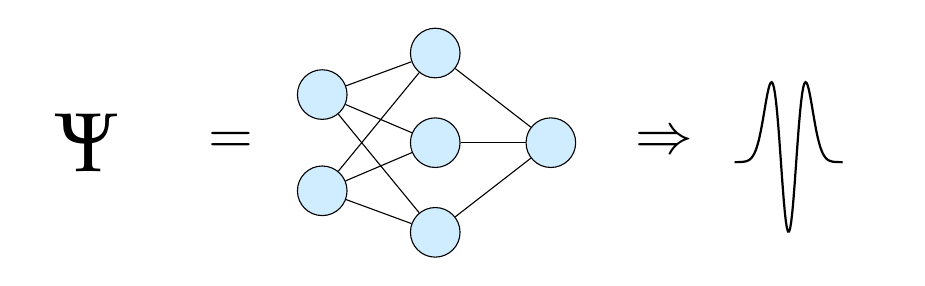
\begin{tikzpicture}

% Neural network
\node[input] (output) {};

\node[input, left=5ex of output] (hidden) {};
\node[input, above=3ex of hidden] (hu) {};
\node[input, below=3ex of hidden] (hl) {};

\node[left=6ex of hidden] (visible) {};
\node[input, above=1ex of visible] (vu) {};
\node[input, below=1ex of visible] (vl) {};

\path[draw] (output) -- (hu);
\path[draw] (output) -- (hidden);
\path[draw] (output) -- (hl);

\path[draw] (vu) -- (hu);
\path[draw] (vu) -- (hidden);
\path[draw] (vu) -- (hl);
\path[draw] (vl) -- (hu);
\path[draw] (vl) -- (hidden);
\path[draw] (vl) -- (hl);

% Wave
\node[right=3ex of output, scale=2] (arrow) {$\Rightarrow$};
\begin{axis}[scale=0.4,
	xshift=10ex, 
	yshift=-8ex, 
	axis line style={draw=none}, 
	ticks=none, 
	xmin=-10,
	xmax=10]
	\addplot[thick, black, samples=100, right=2ex of arrow] plot (\x, { (4*\x*\x - 2) * exp(-0.5 * \x*\x) });
\end{axis}

% Psi
\node[left=3ex of visible, scale=2] (equal) {$=$};
\node[left=3ex of equal, scale=3] {$\Psi$};

\end{tikzpicture}

	\end{figure}
	\begin{itemize}
		\setlength\itemsep{3em}
		\item<3-> Existing methods are reminiscent of machine learning algorithms
		\item<4-> Literature study (\citet{carleo_solving_2017}, \citet{flugsrud_vilde_moe_solving_nodate}, \citet{pfau2019abinitio})
	\end{itemize}
}

\iffalse
\note{No, there are some good reasons. Firstly, neural networks have shown impressive power as function approximators. In quantum mechanical calculations, the so-called wave function contains all the information about the system, and is therefore our ultimate goal to find.  By approximating the wave function by a neural network, the network can in principle provide all the desired information. \bigskip
	
	Secondly, some quantum many-body methods, like the variational Monte Carlo method that we will discuss later, are similar to machine learning techniques. 
	\bigskip
	
	Even though this is a relatively new idea, there exist recent research with the same approach. In 2017, Carlo and Troyer solved the Ising model using restricted Boltzmann machines. A prior student at this group, Flugsrud, extended the work to small quantum dots, and we will again extend her work to larger quantum dots. Recently, Pfau et. al used more traditional neural networks to study atoms and molecules. }
\fi

\mframe{Ethics in Science}{}{
	\begin{itemize}
		\setlength\itemsep{3em}
		\item<1-> Respect for other's work
		\item<2> Reproducibility
		%\item Ethical aspects in machine learning
	\end{itemize}
	\note<1->{
		\begin{itemize}
			\item Whenever others work is used $\rightarrow$ Credit sources $\rightarrow$ text...
			\item When doing experiments $\rightarrow$ Always describe details in a such way
			\item Raw files are available on zenodo
			\item Open source code
		\end{itemize}
	}
}
\titleframe{Quantum Theory}

\note{Now we will give a breif introduction to the essential quantum theory.}

\mframe{The Schrödinger Equation}{}{
	\begin{empheq}[box={\mybluebox[5pt]}]{equation}
	\hat{\mathcal{H}}\Psi=E\Psi
	\end{empheq}
	\pause
	\vspace{0.2cm}
	\begin{center}
		{\large $\Downarrow$}
	\end{center}
	\vspace{0.3cm}
	\begin{equation}
	E=\frac{\int d\bs{X}\Psi^*(\bs{X})\hat{\mathcal{H}}\Psi(\bs{X})}{\int d\bs{X}\Psi^*(\bs{X})\Psi(\bs{X})}
	\end{equation}
	\note<1->{
		\begin{itemize}
			\item Describes the mechanics of all QM systems
			\item Stationary systems $\rightarrow$ Time-independent SE
			\item Linear algebra terms
			\item Configuration interaction
			\item One year on solving 
			\item Difficult to solve bco interactions between particles
		\end{itemize}
	}
}

\iffalse
\note{The Schrödinger equation describes the motion of any quantum mechanical system, and is the equation that I have spent one year solving. Since we will limit us to stationary systems only, the time-independent Schrödinger equation will be our focus. In linear algebra terms, it is an eigenvalue equation with the Hamilton operator, $\hat{\mathcal{H}}$, as a matrix and the wave function, $\Psi$, as the eigen function. $E$ is the energy, which is the eigenvalue.

\vspace{0.5cm}
The most natural way of solving this equation, is to simply express the Hamiltonian as a matrix and obtain the wave function and the energy from diagonalizing the matrix. This is known as configuration interaction. However, we can only do this for small systems, as it is very computational intensive. 
}

\note{Instead, we separate the equation with respect to the energy, and obtain a equation consisting of some integrals. This equation is hard to solve due to the electron-electron correlations. }
\fi

\mframe{The Variational Principle}{}{
	
	
	The variational principle serves as a way of finding the ground state energy. For an arbitrary trial wave function $\Psi_T(\bs{X})$, it states that the obtained energy is larger or equal to the ground state,
	\begin{equation}
	E_0\leq E=\frac{\int d\bs{X}\Psi_T^*(\bs{X})\hat{\mathcal{H}}\Psi_T(\bs{X})}{\int d\bs{X}\Psi_T^*(\bs{X})\Psi_T(\bs{X})}.
	\end{equation}
	Thus, by minimizing the obtained energy, $E$, we can estimate the ground state energy. 
}

\note{
	\begin{itemize}
		\item To obtain the ground state energy
		\item States $\rightarrow$ minimizing
	\end{itemize}
}

\mframe{Quantum Dots}{}{
	Circular quantum dots $\rightarrow$ electrons confined in a harmonic oscillator potential:
	\begin{equation} 		\hat{\mathcal{H}}=\sum_{i=1}^N\left[-\frac{1}{2}\nabla_i^2+\frac{1}{2}\omega^2|\bs{r}_i|^2+\sum_{j>i}^N\frac{1}{r_{ij}}\right].
	\end{equation}
	The number of electrons that give full shells are given by
	\begin{equation}
	N=2\binom{n+d}{d},
	\end{equation}
	which are the magic numbers. 
}

\note{
	\begin{itemize}
		\item Hamiltonian of the circular quantum dots consisting of electrons. In natural units.
		\item The magic numbers give the number of electron in each shell. Looked at closed-shell systems only
	\end{itemize}
}

\titleframe{Machine Learning Theory}

\note{Now over to the machine learning theory. We have already mentioned the artificial neural networks, and we will now look at how they actually work. }

\mframe{Feed-forward Neural Network (FNN)}{}{
	\begin{figure}
		\centering
		\begin{overprint}[9cm]
		\onslide<1>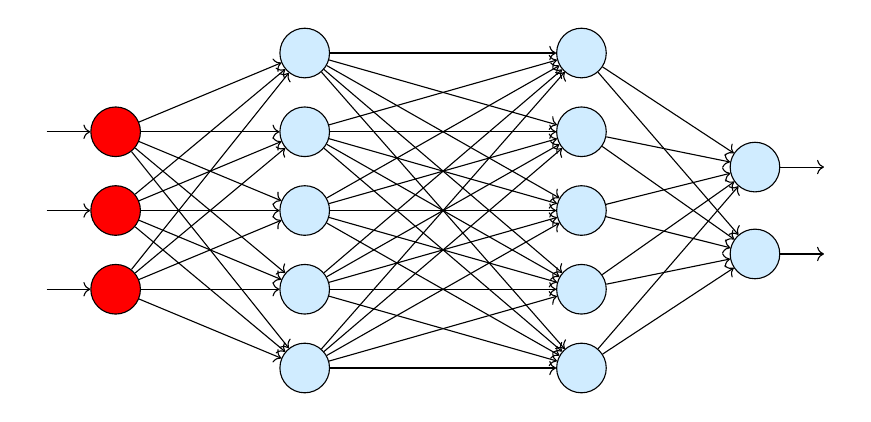
\begin{tikzpicture}

% Define outputs
\node[] (center) {};
\node[input, above=0.3em of center] (y1) {};
\node[input, below=0.3em of center] (y2) {};

% Draw lines from output nodes
\node[right of=y1] (righty1) {};
\node[right of=y2] (righty2) {};
\path[draw,->] (y1) -- (righty1);
\path[draw,->] (y2) -- (righty2);

% Hidden nodes L
\node[input,left=5em of center] (aL3) {};
\node[input,above of=aL3] (aL2) {};
\node[input,above of=aL2] (aL1) {};
\node[input,below of=aL3] (aL4) {};
\node[input,below of=aL4] (aL5) {};

% Hidden nodes 1
\node[input,left=15em of center] (a13) {};
\node[input,above of=a13] (a12) {};
\node[input,above of=a12] (a11) {};
\node[input,below of=a13] (a14) {};
\node[input,below of=a14] (a15) {};

% Draw lines from hidden nodes
\path[draw,->] (aL1) -- (y1);
\path[draw,->] (aL2) -- (y1);
\path[draw,->] (aL3) -- (y1);
\path[draw,->] (aL4) -- (y1);
\path[draw,->] (aL5) -- (y1);

\path[draw,->] (aL1) -- (y2);
\path[draw,->] (aL2) -- (y2);
\path[draw,->] (aL3) -- (y2);
\path[draw,->] (aL4) -- (y2);
\path[draw,->] (aL5) -- (y2);

% Define place left of left
\node[input,left=5em of a13, fill=red] (x2) {};
\node[input,above of=x2, fill=red] (x1) {};
\node[input,below of=x2, fill=red] (x3) {};

% Draw lines from input nodes
\path[draw,->] (x1) -- (a11);
\path[draw,->] (x1) -- (a12);
\path[draw,->] (x1) -- (a13);
\path[draw,->] (x1) -- (a14);
\path[draw,->] (x1) -- (a15);

\path[draw,->] (x2) -- (a11);
\path[draw,->] (x2) -- (a12);
\path[draw,->] (x2) -- (a13);
\path[draw,->] (x2) -- (a14);
\path[draw,->] (x2) -- (a15);

\path[draw,->] (x3) -- (a11);
\path[draw,->] (x3) -- (a12);
\path[draw,->] (x3) -- (a13);
\path[draw,->] (x3) -- (a14);
\path[draw,->] (x3) -- (a15);

% Draw lines from first hidden layer
\path[draw,->] (a11) -- (aL1);
\path[draw,->] (a11) -- (aL2);
\path[draw,->] (a11) -- (aL3);
\path[draw,->] (a11) -- (aL4);
\path[draw,->] (a11) -- (aL5);

\path[draw,->] (a12) -- (aL1);
\path[draw,->] (a12) -- (aL2);
\path[draw,->] (a12) -- (aL3);
\path[draw,->] (a12) -- (aL4);
\path[draw,->] (a12) -- (aL5);

\path[draw,->] (a13) -- (aL1);
\path[draw,->] (a13) -- (aL2);
\path[draw,->] (a13) -- (aL3);
\path[draw,->] (a13) -- (aL4);
\path[draw,->] (a13) -- (aL5);

\path[draw,->] (a14) -- (aL1);
\path[draw,->] (a14) -- (aL2);
\path[draw,->] (a14) -- (aL3);
\path[draw,->] (a14) -- (aL4);
\path[draw,->] (a14) -- (aL5);

\path[draw,->] (a15) -- (aL1);
\path[draw,->] (a15) -- (aL2);
\path[draw,->] (a15) -- (aL3);
\path[draw,->] (a15) -- (aL4);
\path[draw,->] (a15) -- (aL5);


% Draw lines towards input nodes
\node[left of=x1] (leftx1) {};
\node[left of=x2] (leftx2) {};
\node[left of=x3] (leftx3) {};
\path[draw,->] (leftx1) -- (x1);
\path[draw,->] (leftx2) -- (x2);
\path[draw,->] (leftx3) -- (x3); 

\end{tikzpicture}
		\onslide<2>\input{../tikz/multilayer_perceptron_presentation2.tex}
		\onslide<3>\input{../tikz/multilayer_perceptron_presentation3.tex}
		\onslide<4>\input{../tikz/multilayer_perceptron_presentation4.tex}
		\end{overprint}
	\end{figure}
	\hspace{1.45cm}
	\onslide<1-> $\bs{a}_0=\bs{x}$
	\hspace{.95cm}
	\onslide<2-> $\bs{a}_1=f_1(\bs{a}_0)$
	\hspace{1.35cm}
	\onslide<3-> $\bs{a}_2=f_2(\bs{a}_1)$
	\hspace{.35cm}
	\onslide<4-> $\tilde{\bs{y}}=f_3(\bs{a}_2)$
	\note<1->{
		\begin{itemize}
			\item FNNs are among the most popular neural networks
			\item Here a FNN
			\item Many different architectures
			\item Data set $\rightarrow$ propagating
			\item 
		\end{itemize}
	}
}

\mframe{Cost function}{}{
	\begin{itemize}
		\setlength\itemsep{3em}
		\item<1-> The cost function defines the error
		\item<2-> Mean square error (MSE): $$\mathcal{C}=\frac{1}{2}\sum_{i=1}^n(\bs{y}-\tilde{\bs{y}})^2.$$
		\item<3-> Attempt to minimize the cost function
	\end{itemize}
	\note<1->{
		\begin{itemize}
			\item To decide how good the model performs
			\item Continuous model $\rightarrow$ MSE
			\item Want the error to be small $\rightarrow$ minimize the cost function
		\end{itemize}
	}
}

\mframe{Optimization Algorithms}{}{
	\begin{itemize}
		\setlength\itemsep{3em}
		\item<1-> Minimize the cost function
		\item<2-> The gradient descent method: $$\theta^+=\theta-\frac{\partial\mathcal{C}}{\partial\theta}.$$
	\end{itemize}
	\begin{figure}
		\centering
		\begin{overprint}[7cm]
		\onslide<3>\input{../pgf/gradient_minimization1.tex}
		\onslide<4>\input{../pgf/gradient_minimization2.tex}
		\onslide<5>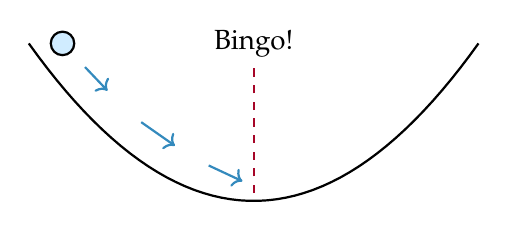
\begin{tikzpicture}[declare function={f(\x)=0.5*\x^2;}]

\newcommand\h{2};			% Particle height
\newcommand\s{1};			% Dashed spacing
\newcommand\X{-2};			% Horizontal position

\begin{axis}[domain=-2:2, samples=50,no markers, hide axis,y=1cm,thick]
\addplot [black] {0.5*x^2};
\node[circle,inner sep=3pt, draw=black, fill=myblue] at (axis cs:-1.7,\h) {};

\draw[->, color=color0] (axis cs:-1.5,1.7) -- (axis cs:-1.3,1.4);
\draw[->, color=color0] (axis cs:-1.,1.) -- (axis cs:-.7,.7);
\draw[->, color=color0] (axis cs:-.4,.45) -- (axis cs:-.1,.25);

\draw[color=color1, dashed]  (axis cs:0,0.1) -- (axis cs:0,1.7);
\node[] at (axis cs:0,2.) {Bingo!};

\end{axis}
\end{tikzpicture}
		\end{overprint}
	\end{figure}
	\note<1->{
		\begin{itemize}
			\item For this, we use optimization algorithms
			\item Plenty of methods $\rightarrow$ tradeoff between simplicity and performance
			\item GD perhaps the simplest $\rightarrow$ move in the direction that minimizes the cost function
			\item We have used the ADAM optimizer, which is slightly more complex. Contains momentum
		\end{itemize}
	}
}

%\note{For the minimization, we use the optimization algorithms which basically find the minimum of any function. There are plenty of different algorithms, which have to tradeoff between simplicity and performance. Perhaps the most basic algorithm is gradient descent, which seeks the minimum based on the gradient. The function is then minimized with respect to the steepest slope, until we have found a minimum. }

\mframe{Find Appropriate Complexity}{}{
	\begin{figure}
		\centering
		% This file was created by tikzplotlib v0.8.1.
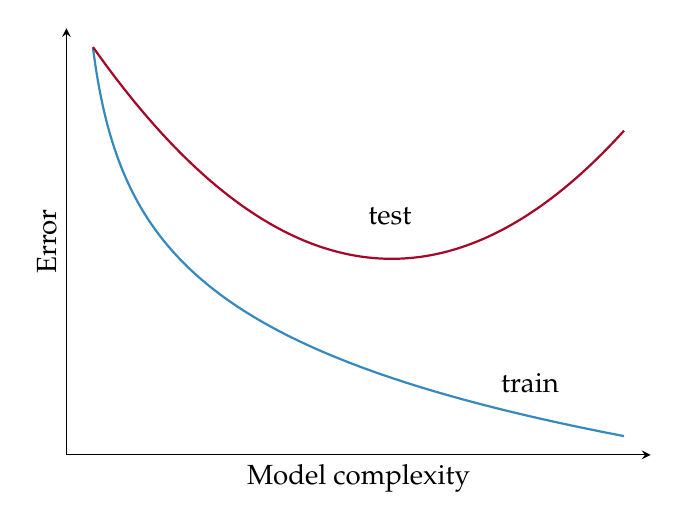
\begin{tikzpicture}

\begin{axis}[
height=7cm, 
width=9cm,
ticks=none,
ylabel near ticks,
xlabel near ticks,
axis x line=bottom,
axis y line=left,
xlabel={Model complexity},
xmin=-0.2, xmax=4.2,
ylabel={Error},
ymin=-16, ymax=4.4
]
\addplot [thick, color0]
table {%
0 3.46573590279973
0.004004004004004 3.26943984054636
0.00800800800800801 3.08055996975182
0.012012012012012 2.89855625448287
0.016016016016016 2.72294557934374
0.02002002002002 2.55329402090492
0.024024024024024 2.38921038789678
0.028028028028028 2.23034078814828
0.032032032032032 2.07636403245592
0.036036036036036 1.92698772528678
0.04004004004004 1.78194492271509
0.044044044044044 1.64099126160566
0.048048048048048 1.5039024824885
0.0520520520520521 1.37047228306363
0.0560560560560561 1.24051045075361
0.0600600600600601 1.11384123187272
0.0640640640640641 0.990301902323346
0.0680680680680681 0.86974151065479
0.0720720720720721 0.752019769128248
0.0760760760760761 0.637006072354703
0.0800800800800801 0.524578626289829
0.0840840840840841 0.414623673020889
0.0880880880880881 0.307034798975167
0.0920920920920921 0.201712316003994
0.0960960960960961 0.0985627063197901
0.1001001001001 -0.00250187645950529
0.104104104104104 -0.101564056829782
0.108108108108108 -0.198701643247571
0.112112112112112 -0.293987995299001
0.116116116116116 -0.387492356531543
0.12012012012012 -0.479280156731312
0.124124124124124 -0.56941328695128
0.128128128128128 -0.657950350185927
0.132132132132132 -0.744946890235164
0.136136136136136 -0.830455600995881
0.14014014014014 -0.914526518155979
0.144144144144144 -0.997207195037107
0.148148148148148 -1.07854286413346
0.152152152152152 -1.15857658572056
0.156156156156156 -1.23734938475645
0.16016016016016 -1.31490037716496
0.164164164164164 -1.39126688647413
0.168168168168168 -1.46648455168055
0.172172172172172 -1.54058742711986
0.176176176176176 -1.61360807504394
0.18018018018018 -1.68557765153477
0.184184184184184 -1.75652598632236
0.188188188188188 -1.82648165701839
0.192192192192192 -1.89547205822808
0.196196196196196 -1.96352346595855
0.2002002002002 -2.03066109770255
0.204204204204204 -2.09690916854147
0.208208208208208 -2.16229094358001
0.212212212212212 -2.22682878699652
0.216216216216216 -2.29054420796793
0.22022022022022 -2.3534579037051
0.224224224224224 -2.41558979981415
0.228228228228228 -2.47695908818075
0.232232232232232 -2.53758426255738
0.236236236236236 -2.59748315201897
0.24024024024024 -2.65667295243809
0.244244244244244 -2.71517025611884
0.248248248248248 -2.77299107971722
0.252252252252252 -2.83015089056543
0.256256256256256 -2.88666463150847
0.26026026026026 -2.94254674435266
0.264264264264264 -2.9978111920183
0.268268268268268 -3.05247147948138
0.272272272272272 -3.10654067358286
0.276276276276276 -3.1600314217784
0.28028028028028 -3.21295596989563
0.284284284284284 -3.26532617896149
0.288288288288288 -3.31715354115734
0.292292292292292 -3.36844919495566
0.296296296296296 -3.41922393948816
0.3003003003003 -3.4694882481916
0.304304304304304 -3.51925228177457
0.308308308308308 -3.5685259005453
0.312312312312312 -3.61731867613791
0.316316316316316 -3.66563990267206
0.32032032032032 -3.71349860737847
0.324324324324324 -3.76090356072069
0.328328328328328 -3.80786328604159
0.332332332332332 -3.85438606876101
0.336336336336336 -3.90047996514947
0.34034034034034 -3.9461528107011
0.344344344344344 -3.99141222812768
0.348348348348348 -4.03626563499401
0.352352352352352 -4.08072025101391
0.356356356356356 -4.12478310502471
0.36036036036036 -4.16846104165712
0.364364364364364 -4.21176072771623
0.368368368368368 -4.25468865828859
0.372372372372372 -4.29725116258944
0.376376376376376 -4.33945440956306
0.38038038038038 -4.38130441324873
0.384384384384384 -4.4228070379241
0.388388388388388 -4.46396800303669
0.392392392392392 -4.50479288793421
0.396396396396396 -4.54528713640318
0.4004004004004 -4.58545606102536
0.404404404404404 -4.6253048473605
0.408408408408408 -4.66483855796373
0.412412412412412 -4.70406213624542
0.416416416416416 -4.74298041018076
0.42042042042042 -4.78159809587608
0.424424424424424 -4.8199198009986
0.428428428428428 -4.85795002807559
0.432432432432432 -4.89569317766909
0.436436436436436 -4.93315355143176
0.44044044044044 -4.97033535504894
0.444444444444444 -5.00724270107231
0.448448448448448 -5.04387961164958
0.452452452452452 -5.08025002115501
0.456456456456456 -5.11635777872485
0.46046046046046 -5.15220665070197
0.464464464464464 -5.18780032299342
0.468468468468468 -5.22314240334467
0.472472472472472 -5.25823642353409
0.476476476476476 -5.29308584149087
0.48048048048048 -5.32769404333971
0.484484484484485 -5.36206434537519
0.488488488488488 -5.39619999596878
0.492492492492492 -5.43010417741113
0.496496496496497 -5.4637800076924
0.500500500500501 -5.49723054222297
0.504504504504504 -5.53045877549701
0.508508508508508 -5.56346764270112
0.512512512512513 -5.59626002127021
0.516516516516517 -5.62883873239272
0.520520520520521 -5.6612065424671
0.524524524524524 -5.69336616451144
0.528528528528528 -5.72532025952805
0.532532532532533 -5.75707143782478
0.536536536536537 -5.78862226029455
0.540540540540541 -5.81997523965481
0.544544544544544 -5.85113284164842
0.548548548548549 -5.88209748620729
0.552552552552553 -5.9128715485802
0.556556556556557 -5.94345736042618
0.560560560560561 -5.97385721087461
0.564564564564565 -6.0040733475533
0.568568568568569 -6.03410797758569
0.572572572572573 -6.06396326855826
0.576576576576577 -6.09364134945928
0.580580580580581 -6.1231443115898
0.584584584584585 -6.15247420944799
0.588588588588589 -6.18163306158758
0.592592592592593 -6.21062285145156
0.596596596596597 -6.23944552818176
0.600600600600601 -6.2681030074052
0.604604604604605 -6.29659717199816
0.608608608608609 -6.32492987282845
0.612612612612613 -6.35310292947687
0.616616616616617 -6.38111813093843
0.620620620620621 -6.40897723630402
0.624624624624625 -6.43668197542321
0.628628628628629 -6.4642340495488
0.632632632632633 -6.49163513196364
0.636636636636637 -6.5188868685905
0.640640640640641 -6.54599087858526
0.644644644644645 -6.57294875491421
0.648648648648649 -6.59976206491584
0.652652652652653 -6.62643235084764
0.656656656656657 -6.65296113041839
0.660660660660661 -6.67934989730643
0.664664664664665 -6.7056001216643
0.668668668668669 -6.73171325061022
0.672672672672673 -6.75769070870678
0.676676676676677 -6.78353389842725
0.680680680680681 -6.80924420060999
0.684684684684685 -6.83482297490112
0.688688688688689 -6.86027156018595
0.692692692692693 -6.88559127500957
0.696696696696697 -6.91078341798675
0.700700700700701 -6.93584926820161
0.704704704704705 -6.96079008559731
0.708708708708709 -6.98560711135605
0.712712712712713 -7.01030156826974
0.716716716716717 -7.03487466110151
0.720720720720721 -7.05932757693839
0.724724724724725 -7.08366148553546
0.728728728728729 -7.10787753965154
0.732732732732733 -7.13197687537695
0.736736736736737 -7.15596061245329
0.740740740740741 -7.17982985458564
0.744744744744745 -7.20358568974734
0.748748748748749 -7.22722919047752
0.752752752752753 -7.25076141417171
0.756756756756757 -7.27418340336556
0.760760760760761 -7.29749618601199
0.764764764764765 -7.32070077575193
0.768768768768769 -7.34379817217873
0.772772772772773 -7.36678936109658
0.776776776776777 -7.38967531477295
0.780780780780781 -7.41245699218531
0.784784784784785 -7.43513533926225
0.788788788788789 -7.45771128911914
0.792792792792793 -7.48018576228854
0.796796796796797 -7.5025596669454
0.800800800800801 -7.52483389912725
0.804804804804805 -7.54700934294956
0.808808808808809 -7.56908687081629
0.812812812812813 -7.59106734362583
0.816816816816817 -7.61295161097244
0.820820820820821 -7.63474051134329
0.824824824824825 -7.65643487231123
0.828828828828829 -7.6780355107234
0.832832832832833 -7.69954323288578
0.836836836836837 -7.72095883474379
0.840840840840841 -7.74228310205901
0.844844844844845 -7.76351681058223
0.848848848848849 -7.78466072622271
0.852852852852853 -7.80571560521403
0.856856856856857 -7.82668219427632
0.860860860860861 -7.84756123077519
0.864864864864865 -7.86835344287735
0.868868868868869 -7.88905954970295
0.872872872872873 -7.90968026147486
0.876876876876877 -7.93021627966481
0.880880880880881 -7.9506682971366
0.884884884884885 -7.97103699828633
0.888888888888889 -7.99132305917988
0.892892892892893 -8.01152714768748
0.896896896896897 -8.0316499236157
0.900900900900901 -8.05169203883675
0.904904904904905 -8.07165413741514
0.908908908908909 -8.0915368557319
0.912912912912913 -8.11134082260631
0.916916916916917 -8.13106665941523
0.920920920920921 -8.1507149802101
0.924924924924925 -8.17028639183159
0.928928928928929 -8.18978149402212
0.932932932932933 -8.20920087953608
0.936936936936937 -8.22854513424802
0.940940940940941 -8.24781483725867
0.944944944944945 -8.267010560999
0.948948948948949 -8.28613287133221
0.952952952952953 -8.30518232765388
0.956956956956957 -8.32415948299008
0.960960960960961 -8.34306488409378
0.964964964964965 -8.36189907153934
0.968968968968969 -8.38066257981523
0.972972972972973 -8.3993559374151
0.976976976976977 -8.41797966692705
0.980980980980981 -8.4365342851213
0.984984984984985 -8.45502030303626
0.988988988988989 -8.47343822606292
0.992992992992993 -8.49178855402784
0.996996996996997 -8.51007178127447
1.001001001001 -8.52828839674309
1.00500500500501 -8.54643888404926
1.00900900900901 -8.56452372156087
1.01301301301301 -8.58254338247375
1.01701701701702 -8.60049833488601
1.02102102102102 -8.61838904187097
1.02502502502503 -8.63621596154884
1.02902902902903 -8.65397954715709
1.03303303303303 -8.67168024711961
1.03703703703704 -8.68931850511461
1.04104104104104 -8.7068947601414
1.04504504504505 -8.72440944658587
1.04904904904905 -8.74186299428499
1.05305305305305 -8.75925582859004
1.05705705705706 -8.77658837042884
1.06106106106106 -8.79386103636689
1.06506506506507 -8.81107423866739
1.06906906906907 -8.82822838535033
1.07307307307307 -8.84532388025052
1.07707707707708 -8.86236112307459
1.08108108108108 -8.8793405094571
1.08508508508509 -8.89626243101569
1.08908908908909 -8.9131272754052
1.09309309309309 -8.92993542637105
1.0970970970971 -8.94668726380154
1.1011011011011 -8.96338316377945
1.10510510510511 -8.98002349863264
1.10910910910911 -8.9966086369839
1.11311311311311 -9.01313894379994
1.11711711711712 -9.0296147804396
1.12112112112112 -9.04603650470119
1.12512512512513 -9.0624044708692
1.12912912912913 -9.07871902976007
1.13313313313313 -9.09498052876738
1.13713713713714 -9.11118931190618
1.14114114114114 -9.12734571985671
1.14514514514515 -9.14345009000733
1.14914914914915 -9.15950275649678
1.15315315315315 -9.17550405025582
1.15715715715716 -9.19145429904814
1.16116116116116 -9.20735382751066
1.16516516516517 -9.22320295719314
1.16916916916917 -9.23900200659725
1.17317317317317 -9.25475129121493
1.17717717717718 -9.27045112356622
1.18118118118118 -9.28610181323647
1.18518518518519 -9.30170366691292
1.18918918918919 -9.31725698842086
1.19319319319319 -9.33276207875901
1.1971971971972 -9.34821923613458
1.2012012012012 -9.3636287559976
1.20520520520521 -9.37899093107487
1.20920920920921 -9.39430605140327
1.21321321321321 -9.40957440436266
1.21721721721722 -9.42479627470821
1.22122122122122 -9.43997194460228
1.22522522522523 -9.45510169364579
1.22922922922923 -9.47018579890914
1.23323323323323 -9.48522453496266
1.23723723723724 -9.50021817390657
1.24124124124124 -9.51516698540055
1.24524524524525 -9.53007123669283
1.24924924924925 -9.54493119264886
1.25325325325325 -9.55974711577953
1.25725725725726 -9.57451926626905
1.26126126126126 -9.5892479020023
1.26526526526527 -9.60393327859188
1.26926926926927 -9.61857564940473
1.27327327327327 -9.63317526558833
1.27727727727728 -9.64773237609659
1.28128128128128 -9.66224722771528
1.28528528528529 -9.67672006508716
1.28928928928929 -9.6911511307367
1.29329329329329 -9.70554066509451
1.2972972972973 -9.7198889065213
1.3013013013013 -9.73419609133163
1.30530530530531 -9.74846245381726
1.30930930930931 -9.76268822627014
1.31331331331331 -9.77687363900513
1.31731731731732 -9.79101892038236
1.32132132132132 -9.80512429682929
1.32532532532533 -9.81918999286248
1.32932932932933 -9.83321623110898
1.33333333333333 -9.84720323232754
1.33733733733734 -9.86115121542939
1.34134134134134 -9.87506039749886
1.34534534534535 -9.8889309938136
1.34934934934935 -9.90276321786461
1.35335335335335 -9.91655728137594
1.35735735735736 -9.93031339432413
1.36136136136136 -9.9440317649574
1.36536536536537 -9.95771259981457
1.36936936936937 -9.97135610374367
1.37337337337337 -9.98496247992044
1.37737737737738 -9.99853192986638
1.38138138138138 -10.0120646534667
1.38538538538539 -10.0255608489881
1.38938938938939 -10.039020713096
1.39339339339339 -10.0524444408717
1.3973973973974 -10.0658322258298
1.4014014014014 -10.0791842599343
1.40540540540541 -10.0925007336156
1.40940940940941 -10.1057818357865
1.41341341341341 -10.1190277538585
1.41741741741742 -10.1322386737576
1.42142142142142 -10.1454147799398
1.42542542542543 -10.1585562554068
1.42942942942943 -10.1716632817211
1.43343343343343 -10.184736039021
1.43743743743744 -10.1977747060356
1.44144144144144 -10.2107794600996
1.44544544544545 -10.2237504771671
1.44944944944945 -10.2366879318269
1.45345345345345 -10.2495919973156
1.45745745745746 -10.2624628455323
1.46146146146146 -10.2753006470518
1.46546546546547 -10.2881055711386
1.46946946946947 -10.3008777857598
1.47347347347347 -10.3136174575987
1.47747747747748 -10.3263247520679
1.48148148148148 -10.3389998333217
1.48548548548549 -10.3516428642696
1.48948948948949 -10.364254006588
1.49349349349349 -10.3768334207332
1.4974974974975 -10.3893812659534
1.5015015015015 -10.4018977003011
1.50550550550551 -10.4143828806444
1.50950950950951 -10.4268369626796
1.51351351351351 -10.4392601009422
1.51751751751752 -10.4516524488187
1.52152152152152 -10.4640141585582
1.52552552552553 -10.4763453812829
1.52952952952953 -10.4886462670001
1.53353353353353 -10.5009169646122
1.53753753753754 -10.5131576219284
1.54154154154154 -10.5253683856747
1.54554554554555 -10.5375494015051
1.54954954954955 -10.5497008140112
1.55355355355355 -10.5618227667332
1.55755755755756 -10.5739154021699
1.56156156156156 -10.5859788617886
1.56556556556557 -10.598013286035
1.56956956956957 -10.6100188143434
1.57357357357357 -10.6219955851457
1.57757757757758 -10.6339437358819
1.58158158158158 -10.6458634030086
1.58558558558559 -10.6577547220091
1.58958958958959 -10.6696178274021
1.59359359359359 -10.6814528527515
1.5975975975976 -10.6932599306745
1.6016016016016 -10.7050391928514
1.60560560560561 -10.7167907700337
1.60960960960961 -10.7285147920535
1.61361361361361 -10.7402113878314
1.61761761761762 -10.7518806853856
1.62162162162162 -10.76352281184
1.62562562562563 -10.7751378934324
1.62962962962963 -10.7867260555231
1.63363363363363 -10.7982874226027
1.63763763763764 -10.8098221183003
1.64164164164164 -10.8213302653911
1.64564564564565 -10.8328119858048
1.64964964964965 -10.8442674006329
1.65365365365365 -10.8556966301366
1.65765765765766 -10.8670997937542
1.66166166166166 -10.8784770101086
1.66566566566567 -10.8898283970149
1.66966966966967 -10.9011540714876
1.67367367367367 -10.9124541497479
1.67767767767768 -10.9237287472305
1.68168168168168 -10.9349779785913
1.68568568568569 -10.9462019577138
1.68968968968969 -10.9574007977166
1.69369369369369 -10.9685746109596
1.6976976976977 -10.9797235090512
1.7017017017017 -10.9908476028549
1.70570570570571 -11.0019470024959
1.70970970970971 -11.0130218173676
1.71371371371371 -11.024072156138
1.71771771771772 -11.0350981267565
1.72172172172172 -11.0460998364595
1.72572572572573 -11.0570773917775
1.72972972972973 -11.0680308985405
1.73373373373373 -11.0789604618848
1.73773773773774 -11.0898661862585
1.74174174174174 -11.100748175428
1.74574574574575 -11.1116065324833
1.74974974974975 -11.1224413598446
1.75375375375375 -11.1332527592675
1.75775775775776 -11.144040831849
1.76176176176176 -11.1548056780331
1.76576576576577 -11.1655473976165
1.76976976976977 -11.176266089754
1.77377377377377 -11.1869618529642
1.77777777777778 -11.1976347851345
1.78178178178178 -11.2082849835273
1.78578578578579 -11.2189125447844
1.78978978978979 -11.2295175649327
1.79379379379379 -11.2401001393896
1.7977977977978 -11.2506603629677
1.8018018018018 -11.2611983298802
1.80580580580581 -11.2717141337459
1.80980980980981 -11.2822078675941
1.81381381381381 -11.2926796238695
1.81781781781782 -11.3031294944375
1.82182182182182 -11.3135575705883
1.82582582582583 -11.3239639430424
1.82982982982983 -11.3343487019549
1.83383383383383 -11.3447119369203
1.83783783783784 -11.3550537369773
1.84184184184184 -11.365374190613
1.84584584584585 -11.3756733857681
1.84984984984985 -11.3859514098405
1.85385385385385 -11.3962083496906
1.85785785785786 -11.4064442916451
1.86186186186186 -11.4166593215018
1.86586586586587 -11.4268535245336
1.86986986986987 -11.437026985493
1.87387387387387 -11.4471797886159
1.87787787787788 -11.4573120176266
1.88188188188188 -11.467423755741
1.88588588588589 -11.4775150856714
1.88988988988989 -11.4875860896301
1.89389389389389 -11.4976368493339
1.8978978978979 -11.5076674460075
1.9019019019019 -11.5176779603879
1.90590590590591 -11.5276684727282
1.90990990990991 -11.5376390628013
1.91391391391391 -11.5475898099037
1.91791791791792 -11.5575207928596
1.92192192192192 -11.5674320900245
1.92592592592593 -11.5773237792885
1.92992992992993 -11.5871959380808
1.93393393393393 -11.5970486433726
1.93793793793794 -11.6068819716809
1.94194194194194 -11.6166959990723
1.94594594594595 -11.6264908011664
1.94994994994995 -11.6362664531391
1.95395395395395 -11.6460230297262
1.95795795795796 -11.6557606052272
1.96196196196196 -11.6654792535079
1.96596596596597 -11.6751790480044
1.96996996996997 -11.6848600617263
1.97397397397397 -11.6945223672599
1.97797797797798 -11.7041660367715
1.98198198198198 -11.7137911420105
1.98598598598599 -11.723397754313
1.98998998998999 -11.7329859446044
1.99399399399399 -11.7425557834031
1.997997997998 -11.7521073408233
2.002002002002 -11.7616406865781
2.00600600600601 -11.7711558899826
2.01001001001001 -11.780653019957
2.01401401401401 -11.7901321450294
2.01801801801802 -11.799593333339
2.02202202202202 -11.8090366526388
2.02602602602603 -11.8184621702987
2.03003003003003 -11.8278699533085
2.03403403403403 -11.8372600682802
2.03803803803804 -11.8466325814515
2.04204204204204 -11.8559875586882
2.04604604604605 -11.8653250654872
2.05005005005005 -11.8746451669788
2.05405405405405 -11.8839479279302
2.05805805805806 -11.8932334127475
2.06206206206206 -11.9025016854788
2.06606606606607 -11.9117528098164
2.07007007007007 -11.9209868491001
2.07407407407407 -11.9302038663191
2.07807807807808 -11.9394039241151
2.08208208208208 -11.9485870847846
2.08608608608609 -11.9577534102814
2.09009009009009 -11.9669029622192
2.09409409409409 -11.9760358018743
2.0980980980981 -11.9851519901875
2.1021021021021 -11.9942515877671
2.10610610610611 -12.003334654891
2.11011011011011 -12.0124012515092
2.11411411411411 -12.0214514372463
2.11811811811812 -12.0304852714035
2.12212212212212 -12.0395028129613
2.12612612612613 -12.0485041205817
2.13013013013013 -12.0574892526101
2.13413413413413 -12.0664582670784
2.13813813813814 -12.0754112217065
2.14214214214214 -12.0843481739048
2.14614614614615 -12.0932691807765
2.15015015015015 -12.1021742991196
2.15415415415415 -12.1110635854292
2.15815815815816 -12.1199370958996
2.16216216216216 -12.1287948864265
2.16616616616617 -12.137637012609
2.17017017017017 -12.1464635297518
2.17417417417417 -12.1552744928672
2.17817817817818 -12.1640699566771
2.18218218218218 -12.1728499756152
2.18618618618619 -12.1816146038291
2.19019019019019 -12.1903638951819
2.19419419419419 -12.1990979032545
2.1981981981982 -12.2078166813477
2.2022022022022 -12.2165202824836
2.20620620620621 -12.2252087594081
2.21021021021021 -12.2338821645927
2.21421421421421 -12.2425405502362
2.21821821821822 -12.2511839682666
2.22222222222222 -12.2598124703432
2.22622622622623 -12.2684261078583
2.23023023023023 -12.277024931939
2.23423423423423 -12.2856089934492
2.23823823823824 -12.2941783429909
2.24224224224224 -12.302733030907
2.24624624624625 -12.3112731072818
2.25025025025025 -12.3197986219438
2.25425425425425 -12.3283096244669
2.25825825825826 -12.3368061641724
2.26226226226226 -12.3452882901305
2.26626626626627 -12.3537560511619
2.27027027027027 -12.3622094958401
2.27427427427427 -12.3706486724922
2.27827827827828 -12.3790736292014
2.28228228228228 -12.3874844138081
2.28628628628629 -12.3958810739115
2.29029029029029 -12.4042636568716
2.29429429429429 -12.4126322098105
2.2982982982983 -12.4209867796143
2.3023023023023 -12.4293274129342
2.30630630630631 -12.4376541561884
2.31031031031031 -12.4459670555637
2.31431431431431 -12.4542661570167
2.31831831831832 -12.4625515062758
2.32232232232232 -12.4708231488422
2.32632632632633 -12.4790811299918
2.33033033033033 -12.4873254947766
2.33433433433433 -12.4955562880258
2.33833833833834 -12.503773554348
2.34234234234234 -12.5119773381319
2.34634634634635 -12.5201676835483
2.35035035035035 -12.528344634551
2.35435435435435 -12.5365082348787
2.35835835835836 -12.5446585280563
2.36236236236236 -12.552795557396
2.36636636636637 -12.560919365999
2.37037037037037 -12.5690299967567
2.37437437437437 -12.5771274923522
2.37837837837838 -12.5852118952615
2.38238238238238 -12.5932832477548
2.38638638638639 -12.601341591898
2.39039039039039 -12.6093869695541
2.39439439439439 -12.617419422384
2.3983983983984 -12.6254389918486
2.4024024024024 -12.6334457192091
2.40640640640641 -12.6414396455292
2.41041041041041 -12.6494208116757
2.41441441441441 -12.6573892583202
2.41841841841842 -12.6653450259401
2.42242242242242 -12.6732881548198
2.42642642642643 -12.6812186850521
2.43043043043043 -12.6891366565394
2.43443443443443 -12.6970421089946
2.43843843843844 -12.7049350819427
2.44244244244244 -12.7128156147218
2.44644644644645 -12.7206837464844
2.45045045045045 -12.7285395161981
2.45445445445445 -12.7363829626475
2.45845845845846 -12.7442141244348
2.46246246246246 -12.752033039981
2.46646646646647 -12.7598397475273
2.47047047047047 -12.7676342851361
2.47447447447447 -12.7754166906918
2.47847847847848 -12.7831870019025
2.48248248248248 -12.7909452563006
2.48648648648649 -12.7986914912439
2.49049049049049 -12.8064257439172
2.49449449449449 -12.8141480513328
2.4984984984985 -12.8218584503317
2.5025025025025 -12.829556977585
2.50650650650651 -12.8372436695943
2.51051051051051 -12.8449185626934
2.51451451451451 -12.8525816930489
2.51851851851852 -12.8602330966615
2.52252252252252 -12.8678728093667
2.52652652652653 -12.8755008668362
2.53053053053053 -12.8831173045784
2.53453453453453 -12.89072215794
2.53853853853854 -12.8983154621064
2.54254254254254 -12.9058972521031
2.54654654654655 -12.9134675627964
2.55055055055055 -12.9210264288945
2.55455455455455 -12.9285738849485
2.55855855855856 -12.9361099653533
2.56256256256256 -12.9436347043483
2.56656656656657 -12.9511481360187
2.57057057057057 -12.9586502942963
2.57457457457457 -12.9661412129602
2.57857857857858 -12.9736209256382
2.58258258258258 -12.9810894658072
2.58658658658659 -12.9885468667944
2.59059059059059 -12.995993161778
2.59459459459459 -13.0034283837883
2.5985985985986 -13.0108525657084
2.6026026026026 -13.0182657402752
2.60660660660661 -13.0256679400801
2.61061061061061 -13.03305919757
2.61461461461461 -13.0404395450483
2.61861861861862 -13.0478090146753
2.62262262262262 -13.0551676384693
2.62662662662663 -13.0625154483078
2.63063063063063 -13.0698524759276
2.63463463463463 -13.0771787529261
2.63863863863864 -13.0844943107621
2.64264264264264 -13.0917991807564
2.64664664664665 -13.0990933940928
2.65065065065065 -13.1063769818188
2.65465465465465 -13.1136499748463
2.65865865865866 -13.1209124039528
2.66266266266266 -13.1281642997815
2.66666666666667 -13.1354056928427
2.67067067067067 -13.1426366135144
2.67467467467467 -13.1498570920427
2.67867867867868 -13.1570671585432
2.68268268268268 -13.1642668430011
2.68668668668669 -13.1714561752725
2.69069069069069 -13.1786351850848
2.69469469469469 -13.1858039020373
2.6986986986987 -13.1929623556027
2.7027027027027 -13.2001105751268
2.70670670670671 -13.2072485898299
2.71071071071071 -13.2143764288075
2.71471471471471 -13.2214941210305
2.71871871871872 -13.2286016953465
2.72272272272272 -13.2356991804802
2.72672672672673 -13.2427866050342
2.73073073073073 -13.2498639974894
2.73473473473473 -13.2569313862063
2.73873873873874 -13.263988799425
2.74274274274274 -13.2710362652663
2.74674674674675 -13.2780738117323
2.75075075075075 -13.285101466707
2.75475475475475 -13.292119257957
2.75875875875876 -13.2991272131321
2.76276276276276 -13.3061253597659
2.76676676676677 -13.3131137252769
2.77077077077077 -13.3200923369684
2.77477477477477 -13.3270612220298
2.77877877877878 -13.3340204075369
2.78278278278278 -13.3409699204524
2.78678678678679 -13.3479097876271
2.79079079079079 -13.3548400357999
2.79479479479479 -13.3617606915988
2.7987987987988 -13.3686717815411
2.8028028028028 -13.3755733320347
2.80680680680681 -13.3824653693781
2.81081081081081 -13.3893479197611
2.81481481481481 -13.3962210092656
2.81881881881882 -13.4030846638662
2.82282282282282 -13.4099389094305
2.82682682682683 -13.4167837717199
2.83083083083083 -13.4236192763903
2.83483483483483 -13.4304454489922
2.83883883883884 -13.437262314972
2.84284284284284 -13.4440698996718
2.84684684684685 -13.4508682283305
2.85085085085085 -13.4576573260843
2.85485485485485 -13.4644372179669
2.85885885885886 -13.4712079289104
2.86286286286286 -13.4779694837459
2.86686686686687 -13.4847219072037
2.87087087087087 -13.4914652239142
2.87487487487487 -13.498199458408
2.87887887887888 -13.5049246351171
2.88288288288288 -13.5116407783748
2.88688688688689 -13.5183479124166
2.89089089089089 -13.5250460613804
2.89489489489489 -13.5317352493074
2.8988988988989 -13.5384155001424
2.9029029029029 -13.5450868377345
2.90690690690691 -13.5517492858371
2.91091091091091 -13.558402868109
2.91491491491491 -13.5650476081149
2.91891891891892 -13.5716835293252
2.92292292292292 -13.5783106551172
2.92692692692693 -13.5849290087756
2.93093093093093 -13.5915386134924
2.93493493493493 -13.5981394923678
2.93893893893894 -13.6047316684109
2.94294294294294 -13.6113151645396
2.94694694694695 -13.6178900035817
2.95095095095095 -13.6244562082746
2.95495495495495 -13.6310138012668
2.95895895895896 -13.6375628051174
2.96296296296296 -13.6441032422971
2.96696696696697 -13.6506351351885
2.97097097097097 -13.6571585060868
2.97497497497497 -13.6636733771997
2.97897897897898 -13.6701797706485
2.98298298298298 -13.6766777084681
2.98698698698699 -13.6831672126076
2.99099099099099 -13.6896483049309
2.99499499499499 -13.6961210072167
2.998998998999 -13.7025853411596
3.003003003003 -13.7090413283698
3.00700700700701 -13.7154889903742
3.01101101101101 -13.7219283486164
3.01501501501502 -13.7283594244572
3.01901901901902 -13.7347822391751
3.02302302302302 -13.7411968139669
3.02702702702703 -13.7476031699475
3.03103103103103 -13.7540013281513
3.03503503503504 -13.7603913095316
3.03903903903904 -13.7667731349616
3.04304304304304 -13.7731468252348
3.04704704704705 -13.7795124010651
3.05105105105105 -13.7858698830876
3.05505505505506 -13.7922192918586
3.05905905905906 -13.7985606478562
3.06306306306306 -13.8048939714808
3.06706706706707 -13.8112192830552
3.07107107107107 -13.8175366028255
3.07507507507508 -13.8238459509607
3.07907907907908 -13.8301473475539
3.08308308308308 -13.8364408126222
3.08708708708709 -13.8427263661072
3.09109109109109 -13.8490040278754
3.0950950950951 -13.8552738177185
3.0990990990991 -13.861535755354
3.1031031031031 -13.8677898604254
3.10710710710711 -13.8740361525023
3.11111111111111 -13.8802746510813
3.11511511511512 -13.8865053755862
3.11911911911912 -13.892728345368
3.12312312312312 -13.8989435797057
3.12712712712713 -13.9051510978065
3.13113113113113 -13.911350918806
3.13513513513514 -13.917543061769
3.13913913913914 -13.9237275456893
3.14314314314314 -13.9299043894904
3.14714714714715 -13.9360736120257
3.15115115115115 -13.942235232079
3.15515515515516 -13.9483892683647
3.15915915915916 -13.9545357395281
3.16316316316316 -13.960674664146
3.16716716716717 -13.9668060607266
3.17117117117117 -13.9729299477103
3.17517517517518 -13.9790463434698
3.17917917917918 -13.9851552663104
3.18318318318318 -13.9912567344705
3.18718718718719 -13.9973507661216
3.19119119119119 -14.003437379369
3.1951951951952 -14.0095165922521
3.1991991991992 -14.0155884227441
3.2032032032032 -14.0216528887533
3.20720720720721 -14.0277100081228
3.21121121121121 -14.0337597986307
3.21521521521522 -14.0398022779908
3.21921921921922 -14.0458374638528
3.22322322322322 -14.0518653738026
3.22722722722723 -14.0578860253624
3.23123123123123 -14.0638994359914
3.23523523523524 -14.0699056230855
3.23923923923924 -14.0759046039785
3.24324324324324 -14.0818963959416
3.24724724724725 -14.0878810161839
3.25125125125125 -14.0938584818529
3.25525525525526 -14.0998288100347
3.25925925925926 -14.1057920177543
3.26326326326326 -14.1117481219757
3.26726726726727 -14.1176971396025
3.27127127127127 -14.1236390874779
3.27527527527528 -14.1295739823852
3.27927927927928 -14.135501841048
3.28328328328328 -14.1414226801306
3.28728728728729 -14.147336516238
3.29129129129129 -14.1532433659164
3.2952952952953 -14.1591432456534
3.2992992992993 -14.1650361718785
3.3033033033033 -14.1709221609628
3.30730730730731 -14.17680122922
3.31131131131131 -14.1826733929062
3.31531531531532 -14.1885386682203
3.31931931931932 -14.1943970713042
3.32332332332332 -14.2002486182431
3.32732732732733 -14.2060933250661
3.33133133133133 -14.2119312077457
3.33533533533534 -14.2177622821988
3.33933933933934 -14.2235865642866
3.34334334334334 -14.2294040698151
3.34734734734735 -14.2352148145348
3.35135135135135 -14.2410188141418
3.35535535535536 -14.2468160842774
3.35935935935936 -14.2526066405284
3.36336336336336 -14.2583904984277
3.36736736736737 -14.2641676734545
3.37137137137137 -14.269938181034
3.37537537537538 -14.2757020365384
3.37937937937938 -14.2814592552867
3.38338338338338 -14.287209852545
3.38738738738739 -14.2929538435268
3.39139139139139 -14.2986912433933
3.3953953953954 -14.3044220672534
3.3993993993994 -14.3101463301644
3.4034034034034 -14.3158640471315
3.40740740740741 -14.321575233109
3.41141141141141 -14.3272799029996
3.41541541541542 -14.3329780716553
3.41941941941942 -14.3386697538773
3.42342342342342 -14.3443549644162
3.42742742742743 -14.3500337179725
3.43143143143143 -14.3557060291965
3.43543543543544 -14.361371912689
3.43943943943944 -14.367031383001
3.44344344344344 -14.372684454634
3.44744744744745 -14.3783311420407
3.45145145145145 -14.3839714596246
3.45545545545546 -14.3896054217407
3.45945945945946 -14.3952330426956
3.46346346346346 -14.4008543367473
3.46746746746747 -14.4064693181061
3.47147147147147 -14.4120780009343
3.47547547547548 -14.4176803993467
3.47947947947948 -14.4232765274106
3.48348348348348 -14.4288663991463
3.48748748748749 -14.434450028527
3.49149149149149 -14.440027429479
3.4954954954955 -14.4455986158823
3.4994994994995 -14.4511636015704
3.5035035035035 -14.4567224003308
3.50750750750751 -14.4622750259049
3.51151151151151 -14.4678214919885
3.51551551551552 -14.4733618122319
3.51951951951952 -14.4788960002398
3.52352352352352 -14.4844240695721
3.52752752752753 -14.4899460337436
3.53153153153153 -14.4954619062244
3.53553553553554 -14.5009717004402
3.53953953953954 -14.5064754297722
3.54354354354354 -14.5119731075574
3.54754754754755 -14.5174647470891
3.55155155155155 -14.5229503616167
3.55555555555556 -14.528429964346
3.55955955955956 -14.5339035684396
3.56356356356356 -14.5393711870166
3.56756756756757 -14.5448328331535
3.57157157157157 -14.5502885198837
3.57557557557558 -14.5557382601982
3.57957957957958 -14.5611820670453
3.58358358358358 -14.5666199533313
3.58758758758759 -14.5720519319204
3.59159159159159 -14.5774780156348
3.5955955955956 -14.582898217255
3.5995995995996 -14.5883125495202
3.6036036036036 -14.593721025128
3.60760760760761 -14.599123656735
3.61161161161161 -14.6045204569567
3.61561561561562 -14.6099114383679
3.61961961961962 -14.6152966135028
3.62362362362362 -14.6206759948549
3.62762762762763 -14.6260495948778
3.63163163163163 -14.6314174259846
3.63563563563564 -14.6367795005488
3.63963963963964 -14.6421358309038
3.64364364364364 -14.6474864293437
3.64764764764765 -14.6528313081231
3.65165165165165 -14.6581704794572
3.65565565565566 -14.6635039555223
3.65965965965966 -14.6688317484556
3.66366366366366 -14.6741538703557
3.66766766766767 -14.6794703332825
3.67167167167167 -14.6847811492575
3.67567567567568 -14.690086330264
3.67967967967968 -14.695385888247
3.68368368368368 -14.7006798351139
3.68768768768769 -14.705968182734
3.69169169169169 -14.7112509429391
3.6956956956957 -14.7165281275236
3.6996996996997 -14.7217997482444
3.7037037037037 -14.7270658168214
3.70770770770771 -14.7323263449376
3.71171171171171 -14.7375813442389
3.71571571571572 -14.7428308263348
3.71971971971972 -14.7480748027981
3.72372372372372 -14.7533132851652
3.72772772772773 -14.7585462849365
3.73173173173173 -14.7637738135759
3.73573573573574 -14.7689958825119
3.73973973973974 -14.7742125031369
3.74374374374374 -14.7794236868078
3.74774774774775 -14.7846294448459
3.75175175175175 -14.7898297885374
3.75575575575576 -14.795024729133
3.75975975975976 -14.8002142778487
3.76376376376376 -14.8053984458654
3.76776776776777 -14.8105772443294
3.77177177177177 -14.8157506843522
3.77577577577578 -14.8209187770111
3.77977977977978 -14.8260815333489
3.78378378378378 -14.8312389643743
3.78778778778779 -14.8363910810619
3.79179179179179 -14.8415378943525
3.7957957957958 -14.8466794151531
3.7997997997998 -14.8518156543372
3.8038038038038 -14.8569466227445
3.80780780780781 -14.8620723311818
3.81181181181181 -14.8671927904225
3.81581581581582 -14.8723080112067
3.81981981981982 -14.877418004242
3.82382382382382 -14.8825227802029
3.82782782782783 -14.8876223497314
3.83183183183183 -14.8927167234368
3.83583583583584 -14.8978059118962
3.83983983983984 -14.9028899256544
3.84384384384384 -14.9079687752239
3.84784784784785 -14.9130424710853
3.85185185185185 -14.9181110236874
3.85585585585586 -14.9231744434472
3.85985985985986 -14.92823274075
3.86386386386386 -14.9332859259498
3.86786786786787 -14.9383340093691
3.87187187187187 -14.9433770012992
3.87587587587588 -14.9484149120002
3.87987987987988 -14.9534477517014
3.88388388388388 -14.9584755306012
3.88788788788789 -14.963498258867
3.89189189189189 -14.968515946636
3.8958958958959 -14.9735286040147
3.8998998998999 -14.9785362410792
3.9039039039039 -14.9835388678753
3.90790790790791 -14.988536494419
3.91191191191191 -14.9935291306959
3.91591591591592 -14.998516786662
3.91991991991992 -15.0034994722434
3.92392392392392 -15.0084771973366
3.92792792792793 -15.0134499718085
3.93193193193193 -15.0184178054967
3.93593593593594 -15.0233807082094
3.93993993993994 -15.0283386897258
3.94394394394394 -15.0332917597957
3.94794794794795 -15.0382399281404
3.95195195195195 -15.043183204452
3.95595595595596 -15.048121598394
3.95995995995996 -15.0530551196014
3.96396396396396 -15.0579837776806
3.96796796796797 -15.0629075822096
3.97197197197197 -15.0678265427381
3.97597597597598 -15.0727406687879
3.97997997997998 -15.0776499698524
3.98398398398398 -15.0825544553973
3.98798798798799 -15.0874541348604
3.99199199199199 -15.0923490176518
3.995995995996 -15.0972391131539
4 -15.1021244307218
};
\addplot [thick, color1]
table {%
0 3.5
0.004004004004004 3.46399602806009
0.00800800800800801 3.42805618431244
0.012012012012012 3.39218046875705
0.016016016016016 3.35636888139391
0.02002002002002 3.32062142222302
0.024024024024024 3.2849380912444
0.028028028028028 3.24931888845803
0.032032032032032 3.21376381386391
0.036036036036036 3.17827286746206
0.04004004004004 3.14284604925246
0.044044044044044 3.10748335923511
0.048048048048048 3.07218479741002
0.0520520520520521 3.03695036377719
0.0560560560560561 3.00178005833661
0.0600600600600601 2.9666738810883
0.0640640640640641 2.93163183203223
0.0680680680680681 2.89665391116843
0.0720720720720721 2.86174011849688
0.0760760760760761 2.82689045401758
0.0800800800800801 2.79210491773054
0.0840840840840841 2.75738350963576
0.0880880880880881 2.72272622973324
0.0920920920920921 2.68813307802297
0.0960960960960961 2.65360405450496
0.1001001001001 2.6191391591792
0.104104104104104 2.5847383920457
0.108108108108108 2.55040175310446
0.112112112112112 2.51612924235547
0.116116116116116 2.48192085979874
0.12012012012012 2.44777660543426
0.124124124124124 2.41369647926204
0.128128128128128 2.37968048128208
0.132132132132132 2.34572861149438
0.136136136136136 2.31184086989893
0.14014014014014 2.27801725649574
0.144144144144144 2.2442577712848
0.148148148148148 2.21056241426612
0.152152152152152 2.17693118543969
0.156156156156156 2.14336408480553
0.16016016016016 2.10986111236362
0.164164164164164 2.07642226811396
0.168168168168168 2.04304755205656
0.172172172172172 2.00973696419142
0.176176176176176 1.97649050451853
0.18018018018018 1.9433081730379
0.184184184184184 1.91018996974953
0.188188188188188 1.87713589465341
0.192192192192192 1.84414594774955
0.196196196196196 1.81122012903795
0.2002002002002 1.7783584385186
0.204204204204204 1.74556087619151
0.208208208208208 1.71282744205667
0.212212212212212 1.68015813611409
0.216216216216216 1.64755295836377
0.22022022022022 1.6150119088057
0.224224224224224 1.58253498743989
0.228228228228228 1.55012219426634
0.232232232232232 1.51777352928504
0.236236236236236 1.485488992496
0.24024024024024 1.45326858389922
0.244244244244244 1.42111230349469
0.248248248248248 1.38902015128241
0.252252252252252 1.3569921272624
0.256256256256256 1.32502823143464
0.26026026026026 1.29312846379914
0.264264264264264 1.26129282435589
0.268268268268268 1.2295213131049
0.272272272272272 1.19781393004616
0.276276276276276 1.16617067517968
0.28028028028028 1.13459154850546
0.284284284284284 1.1030765500235
0.288288288288288 1.07162567973379
0.292292292292292 1.04023893763633
0.296296296296296 1.00891632373114
0.3003003003003 0.977657838018199
0.304304304304304 0.946463480497514
0.308308308308308 0.915333251169088
0.312312312312312 0.884267150032915
0.316316316316316 0.853265177089002
0.32032032032032 0.822327332337343
0.324324324324324 0.791453615777939
0.328328328328328 0.760644027410795
0.332332332332332 0.729898567235904
0.336336336336336 0.699217235253272
0.34034034034034 0.668600031462895
0.344344344344344 0.638046955864773
0.348348348348348 0.60755800845891
0.352352352352352 0.577133189245301
0.356356356356356 0.54677249822395
0.36036036036036 0.516475935394856
0.364364364364364 0.486243500758015
0.368368368368368 0.456075194313432
0.372372372372372 0.425971016061106
0.376376376376376 0.395930966001036
0.38038038038038 0.365955044133223
0.384384384384384 0.336043250457664
0.388388388388388 0.306195584974363
0.392392392392392 0.276412047683318
0.396396396396396 0.24669263858453
0.4004004004004 0.217037357678
0.404404404404404 0.187446204963722
0.408408408408408 0.157919180441702
0.412412412412412 0.128456284111939
0.416416416416416 0.0990575159744331
0.42042042042042 0.0697228760291821
0.424424424424424 0.040452364276188
0.428428428428428 0.0112459807154499
0.432432432432432 -0.0178962746530313
0.436436436436436 -0.0469744018292566
0.44044044044044 -0.0759884008132259
0.444444444444444 -0.104938271604938
0.448448448448448 -0.133824014204395
0.452452452452452 -0.162645628611594
0.456456456456456 -0.191403114826538
0.46046046046046 -0.220096472849225
0.464464464464464 -0.248725702679657
0.468468468468468 -0.277290804317832
0.472472472472472 -0.30579177776375
0.476476476476476 -0.334228623017411
0.48048048048048 -0.362601340078817
0.484484484484485 -0.390909928947967
0.488488488488488 -0.41915438962486
0.492492492492492 -0.447334722109497
0.496496496496497 -0.475450926401877
0.500500500500501 -0.503503002502002
0.504504504504504 -0.531490950409869
0.508508508508508 -0.559414770125481
0.512512512512513 -0.587274461648836
0.516516516516517 -0.615070024979934
0.520520520520521 -0.642801460118777
0.524524524524524 -0.670468767065364
0.528528528528528 -0.698071945819694
0.532532532532533 -0.725610996381767
0.536536536536537 -0.753085918751584
0.540540540540541 -0.780496712929145
0.544544544544544 -0.80784337891445
0.548548548548549 -0.835125916707498
0.552552552552553 -0.86234432630829
0.556556556556557 -0.889498607716825
0.560560560560561 -0.916588760933105
0.564564564564565 -0.94361478595713
0.568568568568569 -0.970576682788896
0.572572572572573 -0.997474451428405
0.576576576576577 -1.02430809187566
0.580580580580581 -1.05107760413066
0.584584584584585 -1.0777829881934
0.588588588588589 -1.10442424406388
0.592592592592593 -1.13100137174211
0.596596596596597 -1.15751437122808
0.600600600600601 -1.1839632425218
0.604604604604605 -1.21034798562326
0.608608608608609 -1.23666860053246
0.612612612612613 -1.26292508724941
0.616616616616617 -1.2891174457741
0.620620620620621 -1.31524567610654
0.624624624624625 -1.34130977824672
0.628628628628629 -1.36730975219464
0.632632632632633 -1.3932455979503
0.636636636636637 -1.41911731551371
0.640640640640641 -1.44492490488487
0.644644644644645 -1.47066836606376
0.648648648648649 -1.4963476990504
0.652652652652653 -1.52196290384479
0.656656656656657 -1.54751398044691
0.660660660660661 -1.57300092885678
0.664664664664665 -1.5984237490744
0.668668668668669 -1.62378244109976
0.672672672672673 -1.64907700493286
0.676676676676677 -1.67430744057371
0.680680680680681 -1.6994737480223
0.684684684684685 -1.72457592727863
0.688688688688689 -1.74961397834271
0.692692692692693 -1.77458790121453
0.696696696696697 -1.79949769589409
0.700700700700701 -1.8243433623814
0.704704704704705 -1.84912490067645
0.708708708708709 -1.87384231077925
0.712712712712713 -1.89849559268979
0.716716716716717 -1.92308474640807
0.720720720720721 -1.9476097719341
0.724724724724725 -1.97207066926787
0.728728728728729 -1.99646743840938
0.732732732732733 -2.02080007935864
0.736736736736737 -2.04506859211564
0.740740740740741 -2.06927297668038
0.744744744744745 -2.09341323305287
0.748748748748749 -2.11748936123311
0.752752752752753 -2.14150136122108
0.756756756756757 -2.1654492330168
0.760760760760761 -2.18933297662026
0.764764764764765 -2.21315259203147
0.768768768768769 -2.23690807925042
0.772772772772773 -2.26059943827712
0.776776776776777 -2.28422666911155
0.780780780780781 -2.30778977175374
0.784784784784785 -2.33128874620366
0.788788788788789 -2.35472359246133
0.792792792792793 -2.37809431052674
0.796796796796797 -2.4014009003999
0.800800800800801 -2.4246433620808
0.804804804804805 -2.44782169556944
0.808808808808809 -2.47093590086583
0.812812812812813 -2.49398597796996
0.816816816816817 -2.51697192688184
0.820820820820821 -2.53989374760146
0.824824824824825 -2.56275144012882
0.828828828828829 -2.58554500446392
0.832832832832833 -2.60827444060677
0.836836836836837 -2.63093974855737
0.840840840840841 -2.6535409283157
0.844844844844845 -2.67607797988178
0.848848848848849 -2.69855090325561
0.852852852852853 -2.72095969843718
0.856856856856857 -2.74330436542649
0.860860860860861 -2.76558490422354
0.864864864864865 -2.78780131482834
0.868868868868869 -2.80995359724088
0.872872872872873 -2.83204175146117
0.876876876876877 -2.8540657774892
0.880880880880881 -2.87602567532498
0.884884884884885 -2.89792144496849
0.888888888888889 -2.91975308641975
0.892892892892893 -2.94152059967876
0.896896896896897 -2.96322398474551
0.900900900900901 -2.98486324162
0.904904904904905 -3.00643837030223
0.908908908908909 -3.02794937079221
0.912912912912913 -3.04939624308994
0.916916916916917 -3.0707789871954
0.920920920920921 -3.09209760310861
0.924924924924925 -3.11335209082957
0.928928928928929 -3.13454245035827
0.932932932932933 -3.15566868169471
0.936936936936937 -3.17673078483889
0.940940940940941 -3.19772875979082
0.944944944944945 -3.21866260655049
0.948948948948949 -3.23953232511791
0.952952952952953 -3.26033791549307
0.956956956956957 -3.28107937767597
0.960960960960961 -3.30175671166662
0.964964964964965 -3.32236991746501
0.968968968968969 -3.34291899507115
0.972972972972973 -3.36340394448502
0.976976976976977 -3.38382476570665
0.980980980980981 -3.40418145873601
0.984984984984985 -3.42447402357312
0.988988988988989 -3.44470246021798
0.992992992992993 -3.46486676867057
0.996996996996997 -3.48496694893091
1.001001001001 -3.505003000999
1.00500500500501 -3.52497492487482
1.00900900900901 -3.5448827205584
1.01301301301301 -3.56472638804971
1.01701701701702 -3.58450592734877
1.02102102102102 -3.60422133845557
1.02502502502503 -3.62387262137012
1.02902902902903 -3.64345977609241
1.03303303303303 -3.66298280262244
1.03703703703704 -3.68244170096022
1.04104104104104 -3.70183647110574
1.04504504504505 -3.72116711305901
1.04904904904905 -3.74043362682001
1.05305305305305 -3.75963601238877
1.05705705705706 -3.77877426976526
1.06106106106106 -3.7978483989495
1.06506506506507 -3.81685839994148
1.06906906906907 -3.83580427274121
1.07307307307307 -3.85468601734868
1.07707707707708 -3.87350363376389
1.08108108108108 -3.89225712198685
1.08508508508509 -3.91094648201755
1.08908908908909 -3.929571713856
1.09309309309309 -3.94813281750219
1.0970970970971 -3.96662979295612
1.1011011011011 -3.9850626402178
1.10510510510511 -4.00343135928722
1.10910910910911 -4.02173595016438
1.11311311311311 -4.03997641284929
1.11711711711712 -4.05815274734194
1.12112112112112 -4.07626495364233
1.12512512512513 -4.09431303175047
1.12912912912913 -4.11229698166635
1.13313313313313 -4.13021680338998
1.13713713713714 -4.14807249692135
1.14114114114114 -4.16586406226046
1.14514514514515 -4.18359149940732
1.14914914914915 -4.20125480836192
1.15315315315315 -4.21885398912426
1.15715715715716 -4.23638904169435
1.16116116116116 -4.25385996607218
1.16516516516517 -4.27126676225775
1.16916916916917 -4.28860943025107
1.17317317317317 -4.30588797005213
1.17717717717718 -4.32310238166094
1.18118118118118 -4.34025266507749
1.18518518518519 -4.35733882030178
1.18918918918919 -4.37436084733382
1.19319319319319 -4.3913187461736
1.1971971971972 -4.40821251682113
1.2012012012012 -4.42504215927639
1.20520520520521 -4.4418076735394
1.20920920920921 -4.45850905961016
1.21321321321321 -4.47514631748866
1.21721721721722 -4.4917194471749
1.22122122122122 -4.50822844866889
1.22522522522523 -4.52467332197062
1.22922922922923 -4.54105406708009
1.23323323323323 -4.55737068399731
1.23723723723724 -4.57362317272227
1.24124124124124 -4.58981153325498
1.24524524524525 -4.60593576559542
1.24924924924925 -4.62199586974362
1.25325325325325 -4.63799184569955
1.25725725725726 -4.65392369346323
1.26126126126126 -4.66979141303466
1.26526526526527 -4.68559500441382
1.26926926926927 -4.70133446760073
1.27327327327327 -4.71700980259539
1.27727727727728 -4.73262100939779
1.28128128128128 -4.74816808800793
1.28528528528529 -4.76365103842581
1.28928928928929 -4.77906986065144
1.29329329329329 -4.79442455468481
1.2972972972973 -4.80971512052593
1.3013013013013 -4.82494155817479
1.30530530530531 -4.8401038676314
1.30930930930931 -4.85520204889574
1.31331331331331 -4.87023610196783
1.31731731731732 -4.88520602684767
1.32132132132132 -4.90011182353525
1.32532532532533 -4.91495349203057
1.32932932932933 -4.92973103233363
1.33333333333333 -4.94444444444444
1.33733733733734 -4.959093728363
1.34134134134134 -4.97367888408929
1.34534534534535 -4.98819991162333
1.34934934934935 -5.00265681096512
1.35335335335335 -5.01704958211465
1.35735735735736 -5.03137822507192
1.36136136136136 -5.04564273983693
1.36536536536537 -5.05984312640969
1.36936936936937 -5.0739793847902
1.37337337337337 -5.08805151497844
1.37737737737738 -5.10205951697443
1.38138138138138 -5.11600339077817
1.38538538538539 -5.12988313638964
1.38938938938939 -5.14369875380886
1.39339339339339 -5.15745024303583
1.3973973973974 -5.17113760407054
1.4014014014014 -5.18476083691299
1.40540540540541 -5.19831994156319
1.40940940940941 -5.21181491802112
1.41341341341341 -5.22524576628681
1.41741741741742 -5.23861248636023
1.42142142142142 -5.2519150782414
1.42542542542543 -5.26515354193032
1.42942942942943 -5.27832787742698
1.43343343343343 -5.29143808473138
1.43743743743744 -5.30448416384352
1.44144144144144 -5.31746611476341
1.44544544544545 -5.33038393749105
1.44944944944945 -5.34323763202642
1.45345345345345 -5.35602719836954
1.45745745745746 -5.3687526365204
1.46146146146146 -5.38141394647901
1.46546546546547 -5.39401112824536
1.46946946946947 -5.40654418181946
1.47347347347347 -5.4190131072013
1.47747747747748 -5.43141790439088
1.48148148148148 -5.4437585733882
1.48548548548549 -5.45603511419327
1.48948948948949 -5.46824752680608
1.49349349349349 -5.48039581122664
1.4974974974975 -5.49247996745494
1.5015015015015 -5.50449999549099
1.50550550550551 -5.51645589533477
1.50950950950951 -5.52834766698631
1.51351351351351 -5.54017531044558
1.51751751751752 -5.5519388257126
1.52152152152152 -5.56363821278736
1.52552552552553 -5.57527347166987
1.52952952952953 -5.58684460236012
1.53353353353353 -5.59835160485811
1.53753753753754 -5.60979447916385
1.54154154154154 -5.62117322527733
1.54554554554555 -5.63248784319855
1.54954954954955 -5.64373833292752
1.55355355355355 -5.65492469446423
1.55755755755756 -5.66604692780869
1.56156156156156 -5.67710503296089
1.56556556556557 -5.68809900992083
1.56956956956957 -5.69902885868852
1.57357357357357 -5.70989457926395
1.57757757757758 -5.72069617164712
1.58158158158158 -5.73143363583804
1.58558558558559 -5.7421069718367
1.58958958958959 -5.75271617964311
1.59359359359359 -5.76326125925726
1.5975975975976 -5.77374221067915
1.6016016016016 -5.78415903390878
1.60560560560561 -5.79451172894616
1.60960960960961 -5.80480029579129
1.61361361361361 -5.81502473444415
1.61761761761762 -5.82518504490476
1.62162162162162 -5.83528122717312
1.62562562562563 -5.84531328124922
1.62962962962963 -5.85528120713306
1.63363363363363 -5.86518500482464
1.63763763763764 -5.87502467432397
1.64164164164164 -5.88480021563105
1.64564564564565 -5.89451162874586
1.64964964964965 -5.90415891366842
1.65365365365365 -5.91374207039873
1.65765765765766 -5.92326109893677
1.66166166166166 -5.93271599928257
1.66566566566567 -5.9421067714361
1.66966966966967 -5.95143341539738
1.67367367367367 -5.9606959311664
1.67767767767768 -5.96989431874317
1.68168168168168 -5.97902857812768
1.68568568568569 -5.98809870931993
1.68968968968969 -5.99710471231993
1.69369369369369 -6.00604658712767
1.6976976976977 -6.01492433374315
1.7017017017017 -6.02373795216638
1.70570570570571 -6.03248744239735
1.70970970970971 -6.04117280443607
1.71371371371371 -6.04979403828253
1.71771771771772 -6.05835114393673
1.72172172172172 -6.06684412139868
1.72572572572573 -6.07527297066837
1.72972972972973 -6.0836376917458
1.73373373373373 -6.09193828463098
1.73773773773774 -6.1001747493239
1.74174174174174 -6.10834708582456
1.74574574574575 -6.11645529413297
1.74974974974975 -6.12449937424912
1.75375375375375 -6.13247932617302
1.75775775775776 -6.14039514990466
1.76176176176176 -6.14824684544404
1.76576576576577 -6.15603441279117
1.76976976976977 -6.16375785194604
1.77377377377377 -6.17141716290865
1.77777777777778 -6.17901234567901
1.78178178178178 -6.18654340025711
1.78578578578579 -6.19401032664296
1.78978978978979 -6.20141312483655
1.79379379379379 -6.20875179483788
1.7977977977978 -6.21602633664696
1.8018018018018 -6.22323675026378
1.80580580580581 -6.23038303568834
1.80980980980981 -6.23746519292065
1.81381381381381 -6.2444832219607
1.81781781781782 -6.25143712280849
1.82182182182182 -6.25832689546403
1.82582582582583 -6.26515253992731
1.82982982982983 -6.27191405619834
1.83383383383383 -6.27861144427711
1.83783783783784 -6.28524470416362
1.84184184184184 -6.29181383585788
1.84584584584585 -6.29831883935988
1.84984984984985 -6.30475971466962
1.85385385385385 -6.31113646178711
1.85785785785786 -6.31744908071234
1.86186186186186 -6.32369757144532
1.86586586586587 -6.32988193398604
1.86986986986987 -6.3360021683345
1.87387387387387 -6.34205827449071
1.87787787787788 -6.34805025245466
1.88188188188188 -6.35397810222635
1.88588588588589 -6.35984182380579
1.88988988988989 -6.36564141719297
1.89389389389389 -6.37137688238789
1.8978978978979 -6.37704821939056
1.9019019019019 -6.38265542820097
1.90590590590591 -6.38819850881913
1.90990990990991 -6.39367746124503
1.91391391391391 -6.39909228547867
1.91791791791792 -6.40444298152006
1.92192192192192 -6.40972954936919
1.92592592592593 -6.41495198902606
1.92992992992993 -6.42011030049068
1.93393393393393 -6.42520448376304
1.93793793793794 -6.43023453884315
1.94194194194194 -6.435200465731
1.94594594594595 -6.44010226442659
1.94994994994995 -6.44493993492993
1.95395395395395 -6.449713477241
1.95795795795796 -6.45442289135983
1.96196196196196 -6.4590681772864
1.96596596596597 -6.46364933502071
1.96996996996997 -6.46816636456276
1.97397397397397 -6.47261926591256
1.97797797797798 -6.4770080390701
1.98198198198198 -6.48133268403539
1.98598598598599 -6.48559320080842
1.98998998998999 -6.48978958938919
1.99399399399399 -6.49392184977771
1.997997997998 -6.49798998197397
2.002002002002 -6.50199398597797
2.00600600600601 -6.50593386178972
2.01001001001001 -6.50980960940921
2.01401401401401 -6.51362122883644
2.01801801801802 -6.51736872007142
2.02202202202202 -6.52105208311415
2.02602602602603 -6.52467131796461
2.03003003003003 -6.52822642462282
2.03403403403403 -6.53171740308877
2.03803803803804 -6.53514425336247
2.04204204204204 -6.53850697544391
2.04604604604605 -6.5418055693331
2.05005005005005 -6.54504003503003
2.05405405405405 -6.5482103725347
2.05805805805806 -6.55131658184711
2.06206206206206 -6.55435866296727
2.06606606606607 -6.55733661589517
2.07007007007007 -6.56025044063082
2.07407407407407 -6.56310013717421
2.07807807807808 -6.56588570552534
2.08208208208208 -6.56860714568422
2.08608608608609 -6.57126445765084
2.09009009009009 -6.57385764142521
2.09409409409409 -6.57638669700732
2.0980980980981 -6.57885162439717
2.1021021021021 -6.58125242359477
2.10610610610611 -6.58358909460011
2.11011011011011 -6.58586163741319
2.11411411411411 -6.58807005203402
2.11811811811812 -6.59021433846259
2.12212212212212 -6.5922944966989
2.12612612612613 -6.59431052674296
2.13013013013013 -6.59626242859476
2.13413413413413 -6.59815020225431
2.13813813813814 -6.5999738477216
2.14214214214214 -6.60173336499663
2.14614614614615 -6.6034287540794
2.15015015015015 -6.60506001496992
2.15415415415415 -6.60662714766819
2.15815815815816 -6.6081301521742
2.16216216216216 -6.60956902848795
2.16616616616617 -6.61094377660944
2.17017017017017 -6.61225439653868
2.17417417417417 -6.61350088827566
2.17817817817818 -6.61468325182039
2.18218218218218 -6.61580148717286
2.18618618618619 -6.61685559433307
2.19019019019019 -6.61784557330103
2.19419419419419 -6.61877142407673
2.1981981981982 -6.61963314666017
2.2022022022022 -6.62043074105136
2.20620620620621 -6.62116420725029
2.21021021021021 -6.62183354525697
2.21421421421421 -6.62243875507139
2.21821821821822 -6.62297983669355
2.22222222222222 -6.62345679012346
2.22622622622623 -6.62386961536111
2.23023023023023 -6.6242183124065
2.23423423423423 -6.62450288125964
2.23823823823824 -6.62472332192052
2.24224224224224 -6.62487963438914
2.24624624624625 -6.62497181866551
2.25025025025025 -6.62499987474962
2.25425425425425 -6.62496380264148
2.25825825825826 -6.62486360234108
2.26226226226226 -6.62469927384842
2.26626626626627 -6.62447081716351
2.27027027027027 -6.62417823228634
2.27427427427427 -6.62382151921691
2.27827827827828 -6.62340067795523
2.28228228228228 -6.62291570850129
2.28628628628629 -6.6223666108551
2.29029029029029 -6.62175338501665
2.29429429429429 -6.62107603098594
2.2982982982983 -6.62033454876298
2.3023023023023 -6.61952893834776
2.30630630630631 -6.61865919974028
2.31031031031031 -6.61772533294055
2.31431431431431 -6.61672733794856
2.31831831831832 -6.61566521476431
2.32232232232232 -6.61453896338781
2.32632632632633 -6.61334858381905
2.33033033033033 -6.61209407605804
2.33433433433433 -6.61077544010477
2.33833833833834 -6.60939267595924
2.34234234234234 -6.60794578362146
2.34634634634635 -6.60643476309142
2.35035035035035 -6.60485961436912
2.35435435435435 -6.60322033745457
2.35835835835836 -6.60151693234776
2.36236236236236 -6.5997493990487
2.36636636636637 -6.59791773755738
2.37037037037037 -6.5960219478738
2.37437437437437 -6.59406202999797
2.37837837837838 -6.59203798392988
2.38238238238238 -6.58994980966953
2.38638638638639 -6.58779750721693
2.39039039039039 -6.58558107657207
2.39439439439439 -6.58330051773495
2.3983983983984 -6.58095583070558
2.4024024024024 -6.57854701548395
2.40640640640641 -6.57607407207007
2.41041041041041 -6.57353700046393
2.41441441441441 -6.57093580066553
2.41841841841842 -6.56827047267488
2.42242242242242 -6.56554101649197
2.42642642642643 -6.5627474321168
2.43043043043043 -6.55988971954938
2.43443443443443 -6.5569678787897
2.43843843843844 -6.55398190983777
2.44244244244244 -6.55093181269357
2.44644644644645 -6.54781758735713
2.45045045045045 -6.54463923382842
2.45445445445445 -6.54139675210746
2.45845845845846 -6.53809014219425
2.46246246246246 -6.53471940408877
2.46646646646647 -6.53128453779104
2.47047047047047 -6.52778554330106
2.47447447447447 -6.52422242061882
2.47847847847848 -6.52059516974432
2.48248248248248 -6.51690379067756
2.48648648648649 -6.51314828341855
2.49049049049049 -6.50932864796729
2.49449449449449 -6.50544488432376
2.4984984984985 -6.50149699248798
2.5025025025025 -6.49748497245995
2.50650650650651 -6.49340882423965
2.51051051051051 -6.48926854782711
2.51451451451451 -6.4850641432223
2.51851851851852 -6.48079561042524
2.52252252252252 -6.47646294943592
2.52652652652653 -6.47206616025435
2.53053053053053 -6.46760524288052
2.53453453453453 -6.46308019731443
2.53853853853854 -6.45849102355609
2.54254254254254 -6.45383772160549
2.54654654654655 -6.44912029146263
2.55055055055055 -6.44433873312752
2.55455455455455 -6.43949304660015
2.55855855855856 -6.43458323188053
2.56256256256256 -6.42960928896865
2.56656656656657 -6.42457121786451
2.57057057057057 -6.41946901856812
2.57457457457457 -6.41430269107947
2.57857857857858 -6.40907223539856
2.58258258258258 -6.4037776515254
2.58658658658659 -6.39841893945998
2.59059059059059 -6.39299609920231
2.59459459459459 -6.38750913075237
2.5985985985986 -6.38195803411019
2.6026026026026 -6.37634280927574
2.60660660660661 -6.37066345624904
2.61061061061061 -6.36491997503009
2.61461461461461 -6.35911236561887
2.61861861861862 -6.3532406280154
2.62262262262262 -6.34730476221968
2.62662662662663 -6.3413047682317
2.63063063063063 -6.33524064605146
2.63463463463463 -6.32911239567896
2.63863863863864 -6.32292001711421
2.64264264264264 -6.3166635103572
2.64664664664665 -6.31034287540794
2.65065065065065 -6.30395811226642
2.65465465465465 -6.29750922093264
2.65865865865866 -6.29099620140661
2.66266266266266 -6.28441905368832
2.66666666666667 -6.27777777777778
2.67067067067067 -6.27107237367498
2.67467467467467 -6.26430284137992
2.67867867867868 -6.2574691808926
2.68268268268268 -6.25057139221303
2.68668668668669 -6.24360947534121
2.69069069069069 -6.23658343027712
2.69469469469469 -6.22949325702078
2.6986986986987 -6.22233895557219
2.7027027027027 -6.21512052593134
2.70670670670671 -6.20783796809823
2.71071071071071 -6.20049128207286
2.71471471471471 -6.19308046785524
2.71871871871872 -6.18560552544537
2.72272272272272 -6.17806645484323
2.72672672672673 -6.17046325604884
2.73073073073073 -6.1627959290622
2.73473473473473 -6.15506447388329
2.73873873873874 -6.14726889051213
2.74274274274274 -6.13940917894872
2.74674674674675 -6.13148533919305
2.75075075075075 -6.12349737124512
2.75475475475475 -6.11544527510493
2.75875875875876 -6.10732905077249
2.76276276276276 -6.0991486982478
2.76676676676677 -6.09090421753084
2.77077077077077 -6.08259560862163
2.77477477477477 -6.07422287152017
2.77877877877878 -6.06578600622645
2.78278278278278 -6.05728501274047
2.78678678678679 -6.04871989106223
2.79079079079079 -6.04009064119174
2.79479479479479 -6.03139726312899
2.7987987987988 -6.02263975687399
2.8028028028028 -6.01381812242673
2.80680680680681 -6.00493235978722
2.81081081081081 -5.99598246895544
2.81481481481481 -5.98696844993141
2.81881881881882 -5.97789030271513
2.82282282282282 -5.96874802730659
2.82682682682683 -5.95954162370579
2.83083083083083 -5.95027109191273
2.83483483483483 -5.94093643192742
2.83883883883884 -5.93153764374986
2.84284284284284 -5.92207472738003
2.84684684684685 -5.91254768281795
2.85085085085085 -5.90295651006362
2.85485485485485 -5.89330120911703
2.85885885885886 -5.88358177997818
2.86286286286286 -5.87379822264707
2.86686686686687 -5.86395053712371
2.87087087087087 -5.85403872340809
2.87487487487487 -5.84406278150022
2.87887887887888 -5.83402271140009
2.88288288288288 -5.8239185131077
2.88688688688689 -5.81375018662306
2.89089089089089 -5.80351773194616
2.89489489489489 -5.793221149077
2.8988988988989 -5.78286043801559
2.9029029029029 -5.77243559876193
2.90690690690691 -5.761946631316
2.91091091091091 -5.75139353567782
2.91491491491491 -5.74077631184738
2.91891891891892 -5.73009495982469
2.92292292292292 -5.71934947960974
2.92692692692693 -5.70853987120253
2.93093093093093 -5.69766613460307
2.93493493493493 -5.68672826981135
2.93893893893894 -5.67572627682738
2.94294294294294 -5.66466015565115
2.94694694694695 -5.65352990628266
2.95095095095095 -5.64233552872192
2.95495495495495 -5.63107702296892
2.95895895895896 -5.61975438902366
2.96296296296296 -5.60836762688615
2.96696696696697 -5.59691673655638
2.97097097097097 -5.58540171803435
2.97497497497497 -5.57382257132007
2.97897897897898 -5.56217929641353
2.98298298298298 -5.55047189331474
2.98698698698699 -5.53870036202368
2.99099099099099 -5.52686470254038
2.99499499499499 -5.51496491486481
2.998998998999 -5.503000998997
3.003003003003 -5.49097295493692
3.00700700700701 -5.47888078268459
3.01101101101101 -5.46672448224
3.01501501501502 -5.45450405360315
3.01901901901902 -5.44221949677405
3.02302302302302 -5.42987081175269
3.02702702702703 -5.41745799853908
3.03103103103103 -5.40498105713321
3.03503503503504 -5.39243998753508
3.03903903903904 -5.3798347897447
3.04304304304304 -5.36716546376206
3.04704704704705 -5.35443200958716
3.05105105105105 -5.34163442722001
3.05505505505506 -5.3287727166606
3.05905905905906 -5.31584687790894
3.06306306306306 -5.30285691096502
3.06706706706707 -5.28980281582884
3.07107107107107 -5.27668459250041
3.07507507507508 -5.26350224097972
3.07907907907908 -5.25025576126677
3.08308308308308 -5.23694515336157
3.08708708708709 -5.22357041726411
3.09109109109109 -5.2101315529744
3.0950950950951 -5.19662856049242
3.0990990990991 -5.1830614398182
3.1031031031031 -5.16943019095171
3.10710710710711 -5.15573481389297
3.11111111111111 -5.14197530864197
3.11511511511512 -5.12815167519872
3.11911911911912 -5.11426391356321
3.12312312312312 -5.10031202373545
3.12712712712713 -5.08629600571542
3.13113113113113 -5.07221585950315
3.13513513513514 -5.05807158509861
3.13913913913914 -5.04386318250182
3.14314314314314 -5.02959065171278
3.14714714714715 -5.01525399273147
3.15115115115115 -5.00085320555791
3.15515515515516 -4.98638829019209
3.15915915915916 -4.97185924663402
3.16316316316316 -4.95726607488369
3.16716716716717 -4.94260877494111
3.17117117117117 -4.92788734680627
3.17517517517518 -4.91310179047917
3.17917917917918 -4.89825210595981
3.18318318318318 -4.8833382932482
3.18718718718719 -4.86836035234434
3.19119119119119 -4.85331828324821
3.1951951951952 -4.83821208595983
3.1991991991992 -4.8230417604792
3.2032032032032 -4.80780730680631
3.20720720720721 -4.79250872494116
3.21121121121121 -4.77714601488375
3.21521521521522 -4.76171917663409
3.21921921921922 -4.74622821019218
3.22322322322322 -4.730673115558
3.22722722722723 -4.71505389273157
3.23123123123123 -4.69937054171288
3.23523523523524 -4.68362306250194
3.23923923923924 -4.66781145509874
3.24324324324324 -4.65193571950329
3.24724724724725 -4.63599585571558
3.25125125125125 -4.61999186373561
3.25525525525526 -4.60392374356338
3.25925925925926 -4.5877914951989
3.26326326326326 -4.57159511864216
3.26726726726727 -4.55533461389317
3.27127127127127 -4.53900998095192
3.27527527527528 -4.52262121981842
3.27927927927928 -4.50616833049266
3.28328328328328 -4.48965131297464
3.28728728728729 -4.47307016726436
3.29129129129129 -4.45642489336183
3.2952952952953 -4.43971549126704
3.2992992992993 -4.42294196098
3.3033033033033 -4.4061043025007
3.30730730730731 -4.38920251582914
3.31131131131131 -4.37223660096533
3.31531531531532 -4.35520655790926
3.31931931931932 -4.33811238666094
3.32332332332332 -4.32095408722035
3.32732732732733 -4.30373165958752
3.33133133133133 -4.28644510376242
3.33533533533534 -4.26909441974507
3.33933933933934 -4.25167960753546
3.34334334334334 -4.2342006671336
3.34734734734735 -4.21665759853948
3.35135135135135 -4.19905040175311
3.35535535535536 -4.18137907677447
3.35935935935936 -4.16364362360358
3.36336336336336 -4.14584404224044
3.36736736736737 -4.12798033268504
3.37137137137137 -4.11005249493738
3.37537537537538 -4.09206052899747
3.37937937937938 -4.0740044348653
3.38338338338338 -4.05588421254087
3.38738738738739 -4.03769986202419
3.39139139139139 -4.01945138331525
3.3953953953954 -4.00113877641405
3.3993993993994 -3.9827620413206
3.4034034034034 -3.96432117803489
3.40740740740741 -3.94581618655693
3.41141141141141 -3.92724706688671
3.41541541541542 -3.90861381902423
3.41941941941942 -3.8899164429695
3.42342342342342 -3.87115493872251
3.42742742742743 -3.85232930628326
3.43143143143143 -3.83343954565176
3.43543543543544 -3.814485656828
3.43943943943944 -3.79546763981199
3.44344344344344 -3.77638549460371
3.44744744744745 -3.75723922120318
3.45145145145145 -3.7380288196104
3.45545545545546 -3.71875428982536
3.45945945945946 -3.69941563184806
3.46346346346346 -3.68001284567851
3.46746746746747 -3.6605459313167
3.47147147147147 -3.64101488876264
3.47547547547548 -3.62141971801632
3.47947947947948 -3.60176041907774
3.48348348348348 -3.5820369919469
3.48748748748749 -3.56224943662381
3.49149149149149 -3.54239775310846
3.4954954954955 -3.52248194140086
3.4994994994995 -3.502502001501
3.5035035035035 -3.48245793340888
3.50750750750751 -3.46234973712451
3.51151151151151 -3.44217741264788
3.51551551551552 -3.421940959979
3.51951951951952 -3.40164037911786
3.52352352352352 -3.38127567006446
3.52752752752753 -3.3608468328188
3.53153153153153 -3.3403538673809
3.53553553553554 -3.31979677375073
3.53953953953954 -3.2991755519283
3.54354354354354 -3.27849020191362
3.54754754754755 -3.25774072370669
3.55155155155155 -3.2369271173075
3.55555555555556 -3.21604938271605
3.55955955955956 -3.19510751993234
3.56356356356356 -3.17410152895638
3.56756756756757 -3.15303140978817
3.57157157157157 -3.13189716242769
3.57557557557558 -3.11069878687496
3.57957957957958 -3.08943628312998
3.58358358358358 -3.06810965119273
3.58758758758759 -3.04671889106324
3.59159159159159 -3.02526400274148
3.5955955955956 -3.00374498622747
3.5995995995996 -2.9821618415212
3.6036036036036 -2.96051456862268
3.60760760760761 -2.9388031675319
3.61161161161161 -2.91702763824886
3.61561561561562 -2.89518798077357
3.61961961961962 -2.87328419510602
3.62362362362362 -2.85131628124621
3.62762762762763 -2.82928423919415
3.63163163163163 -2.80718806894983
3.63563563563564 -2.78502777051326
3.63963963963964 -2.76280334388442
3.64364364364364 -2.74051478906334
3.64764764764765 -2.71816210604999
3.65165165165165 -2.6957452948444
3.65565565565566 -2.67326435544654
3.65965965965966 -2.65071928785642
3.66366366366366 -2.62811009207406
3.66766766766767 -2.60543676809943
3.67167167167167 -2.58269931593255
3.67567567567568 -2.55989773557341
3.67967967967968 -2.53703202702202
3.68368368368368 -2.51410219027837
3.68768768768769 -2.49110822534246
3.69169169169169 -2.4680501322143
3.6956956956957 -2.44492791089388
3.6996996996997 -2.4217415613812
3.7037037037037 -2.39849108367627
3.70770770770771 -2.37517647777908
3.71171171171171 -2.35179774368964
3.71571571571572 -2.32835488140794
3.71971971971972 -2.30484789093398
3.72372372372372 -2.28127677226776
3.72772772772773 -2.25764152540929
3.73173173173173 -2.23394215035857
3.73573573573574 -2.21017864711558
3.73973973973974 -2.18635101568034
3.74374374374374 -2.16245925605285
3.74774774774775 -2.1385033682331
3.75175175175175 -2.11448335222109
3.75575575575576 -2.09039920801682
3.75975975975976 -2.0662509356203
3.76376376376376 -2.04203853503153
3.76776776776777 -2.0177620062505
3.77177177177177 -1.99342134927721
3.77577577577578 -1.96901656411166
3.77977977977978 -1.94454765075386
3.78378378378378 -1.9200146092038
3.78778778778779 -1.89541743946148
3.79179179179179 -1.87075614152691
3.7957957957958 -1.84603071540008
3.7997997997998 -1.821241161081
3.8038038038038 -1.79638747856966
3.80780780780781 -1.77146966786607
3.81181181181181 -1.74648772897021
3.81581581581582 -1.7214416618821
3.81981981981982 -1.69633146660174
3.82382382382382 -1.67115714312912
3.82782782782783 -1.64591869146424
3.83183183183183 -1.6206161116071
3.83583583583584 -1.59524940355771
3.83983983983984 -1.56981856731606
3.84384384384384 -1.54432360288216
3.84784784784785 -1.518764510256
3.85185185185185 -1.49314128943759
3.85585585585586 -1.46745394042691
3.85985985985986 -1.44170246322398
3.86386386386386 -1.4158868578288
3.86786786786787 -1.39000712424136
3.87187187187187 -1.36406326246166
3.87587587587588 -1.33805527248971
3.87987987987988 -1.3119831543255
3.88388388388388 -1.28584690796903
3.88788788788789 -1.25964653342031
3.89189189189189 -1.23338203067933
3.8958958958959 -1.20705339974609
3.8998998998999 -1.1806606406206
3.9039039039039 -1.15420375330285
3.90790790790791 -1.12768273779285
3.91191191191191 -1.10109759409059
3.91591591591592 -1.07444832219607
3.91991991991992 -1.0477349221093
3.92392392392392 -1.02095739383027
3.92792792792793 -0.994115737358982
3.93193193193193 -0.96720995269544
3.93593593593594 -0.940240039839639
3.93993993993994 -0.913205998791584
3.94394394394394 -0.886107829551273
3.94794794794795 -0.858945532118707
3.95195195195195 -0.831719106493883
3.95595595595596 -0.8044285526768
3.95995995995996 -0.777073870667464
3.96396396396396 -0.749655060465872
3.96796796796797 -0.722172122072023
3.97197197197197 -0.694625055485915
3.97597597597598 -0.667013860707554
3.97997997997998 -0.639338537736936
3.98398398398398 -0.611599086574062
3.98798798798799 -0.583795507218932
3.99199199199199 -0.555927799671542
3.995995995996 -0.527995963931899
4 -0.5
};
\node at (axis cs:2,-5)[
  %scale=0.5,
  anchor=base west,
  text=black,
  rotate=0.0
]{test};
\node at (axis cs:3,-13)[
  %scale=0.5,
  anchor=base west,
  text=black,
  rotate=0.0
]{train};
\end{axis}

\end{tikzpicture}
	\end{figure}
}

\note{
	\begin{itemize}
		\item Different architectures with different complexities
		\item Spkit data set in training and test set
		\item Want to minimize test error $\rightarrow$ trial and error
	\end{itemize}
}

\mframe{Restricted Boltzmann Machines}{}{
	\begin{figure}
		\centering
		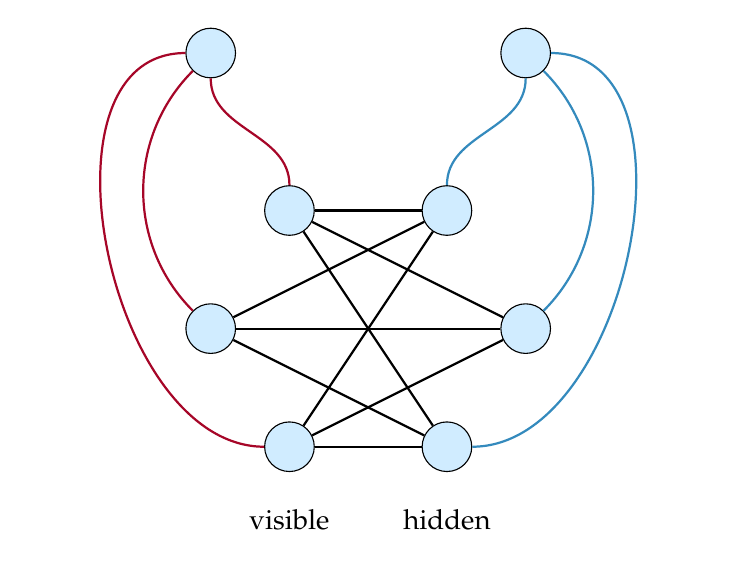
\begin{tikzpicture}

% Define visible units
\node[input] (x2) {};
\node[input] at (1,+3/2) (x1) {};
\node[input] at (1,-3/2) (x3) {};

% Define hidden units
\node[input] at (3,+3/2) (h1) {};
\node[input] at (4,0) (h2) {};
\node[input] at (3,-3/2) (h3) {};

% Define biases
\node[input] at (0,7/2) (a) {};
\node[input] at (4,7/2) (b) {};

% Define paths
\path[draw,thick,-] (x1) -- (h1);
\path[draw,thick,-] (x1) -- (h2);
\path[draw,thick,-] (x1) -- (h3);

\path[draw,thick,-] (x2) -- (h1);
\path[draw,thick,-] (x2) -- (h2);
\path[draw,thick,-] (x2) -- (h3);

\path[draw,thick,-] (x3) -- (h1);
\path[draw,thick,-] (x3) -- (h2);
\path[draw,thick,-] (x3) -- (h3);

\draw[color0,thick,-] (b) to [out=270,in=90] (h1);
\draw[color0,thick,-] (b) to [out=315,in=45] (h2);
\draw[color0,thick,-] (b) to [out=0,in=0] (h3);

\draw[color1,thick,-] (a) to [out=270,in=90] (x1);
\draw[color1,thick,-] (a) to [out=225,in=135] (x2);
\draw[color1,thick,-] (a) to  [out=180,in=180] (x3);


% Add some text
\node[below=1em of x3] {visible};
\node[below=1em of h3] {hidden};
\end{tikzpicture}

	\end{figure}
	\pause
	\begin{equation}
	E(\bs{x},\bs{h})=-\sum_{i=1}^V\frac{(x_i-a_i)^2}{2\sigma_i^2}-\sum_{j=1}^Hh_jb_j-\sum_{i=1}^V\sum_{j=1}^H\frac{x_iw_{ij}h_j}{\sigma_i^2}
	\end{equation}
}

\note{
	\begin{itemize}
		\item What we have used in our work
		\item Energy based model
		\item Differs from FNN $\rightarrow$ obey unsupervised $\rightarrow$ no labeled data
		\item Finds the most likely configuration by minimizing the system energy
	\end{itemize}
}

\mframe{Probability Distribution}{}{
	The joint probability distribution is given by the Boltzmann distribution:
	
	\begin{equation}
	P(\bs{x},\bs{h})=\frac{1}{Z}\exp(-E(\bs{x},\bs{h})/kT).
	\end{equation}
	The marginal distribution of the visible units is given by
	\begin{equation}
	P(\bs{x})=\sum_{\{\bs{h}\}}P(\bs{x},\bs{h}).
	\end{equation}
}

\note{
	\begin{itemize}
		\item Named Boltzmann machine because of the joint probability distribution
		\item Find the marginal distribution of the visible units by integrating over all the hidden units
	\end{itemize}
}
\titleframe{Methods}

\note{The applied methods will be discussed briefly}

\mframe{Variational Monte Carlo (VMC)}{}{
	Exploit the variational principle in order to obtain the ground state energy
	\begin{equation}
	\begin{aligned}
	E_0 < E_{\text{VMC}} &= \frac{\int d\bs{R}\Psi_T(\bs{R})^*\hat{\mathcal{H}}\Psi_T(\bs{R})}{\int d\bs{R}\Psi_T(\bs{R})^*\Psi_T(\bs{R})},\\
	%&= \int d\bs{R}\underbrace{\frac{\Psi_T(\bs{R})^*\Psi_T(\bs{R})}{\int d\bs{R}\Psi_T(\bs{R})^*\Psi_T(\bs{R})}}_{P(\bs{R})}\cdot\underbrace{\frac{1}{\Psi_T(\bs{R})}\hat{\mathcal{H}}\Psi_T(\bs{R})}_{E_L(\bs{R})}\\
	&=\int d\bs{R}E_L(\bs{R})P(\bs{R}),
	\end{aligned}
	\end{equation}
	with
	\begin{equation}
	E_L(\bs{R})=\frac{1}{\Psi_T(\bs{R})}\hat{\mathcal{H}}\Psi_T(\bs{R})\quad\wedge\quad P(\bs{R})=\frac{\Psi_T(\bs{R})^*\Psi_T(\bs{R})}{\int d\bs{R}\Psi_T(\bs{R})^*\Psi_T(\bs{R})}
	\end{equation}
}

\note{
	\begin{itemize}
		\item Our work is based on VMC
		\item Exploits variational principle
		\item We start with rewriting the expression in terms of the local energy and the probability density function
	\end{itemize}
}

\mframe{Monte Carlo Integration}{}{
	We attempt to solve the integral by sampling from the probability density function $P(\bs{R})\propto\Psi_T(\bs{R})^*\Psi_T(\bs{R})$:
	\begin{equation}
	\begin{aligned}
	E_{\text{VMC}} &= \int d\bs{R} E_L(\bs{R})P(\bs{R}),\\
	&\approx\frac{1}{M}\sum_{i=1}^ME_L(\bs{R}_i).
	\end{aligned}
	\end{equation}
}

\note{
	\begin{itemize}
		\item The reason $\rightarrow$ On the form of a general expectation value
		\item Can be solved by Monte Carlo integration
		\item Only gives an energy
		\item Find the ground state energy by adjusting the trial wave fucntion with respect to minimizing the energy. Repeat exercise. When the energy has converged, we have a ground state energy estimate.
	\end{itemize}
}

\mframe{Trial Wave Function Ansatz}{}{
	
	The Slater-Jastrow function is the \textit{de facto} standard trial wave function for electronic structure systems,
	\begin{equation}
	\Psi_T(\bs{R})=|\hat{D}(\bs{R})|J(\bs{R}),
	\end{equation}
	where the Slater matrix,
	\begin{equation}
	\hat{D}(\bs{R})=
	\begin{pmatrix}
	\phi_1(\boldsymbol{r}_1) & \phi_2(\boldsymbol{r}_1) & \hdots & \phi_N(\boldsymbol{r}_1)\\
	\phi_1(\boldsymbol{r}_2) & \phi_2(\boldsymbol{r}_2) & \hdots & \phi_N(\boldsymbol{r}_2)\\
	\vdots & \vdots & \ddots & \vdots \\
	\phi_1(\boldsymbol{r}_N) & \phi_2(\boldsymbol{r}_N) & \hdots & \phi_N(\boldsymbol{r}_N)
	\end{pmatrix},
	\end{equation}
	contains all the single-particle functions.
}

\note{
	\begin{itemize}
		\item Arbitrary function $\rightarrow$ Few requirements $\rightarrow$ electron systems
		\item Standard Slater-Jastrow function
	\end{itemize}
}

\mframe{Single-particle Functions}{}{
	The Hermite functions,
	\begin{equation}
	\phi_n(\bs{r})\propto H_n(\sqrt{\omega}\bs{r})\exp(-\frac{1}{2}\alpha\omega|\bs{r}|^2),
	\end{equation}
	are often used as the single-particle functions for quantum dots. The Gaussian can be factorized out from the Slater determinant,
	\begin{equation}
	|\hat{D}(\bs{R};\alpha)|\propto\exp(-\frac{1}{2}\alpha\omega|\bs{R}|^2)
	\begin{vmatrix}
	H_1(\boldsymbol{r}_1) & H_2(\boldsymbol{r}_1) & \hdots & H_N(\boldsymbol{r}_1)\\
	H_1(\boldsymbol{r}_2) & H_2(\boldsymbol{r}_2) & \hdots & H_N(\boldsymbol{r}_2)\\
	\vdots & \vdots & \ddots & \vdots \\
	H_1(\boldsymbol{r}_N) & H_2(\boldsymbol{r}_N) & \hdots & H_N(\boldsymbol{r}_N)
	\end{vmatrix}.
	\end{equation}
}

\note{
	\begin{itemize}
		\item Hermite functions often used for circular quantum dots $\rightarrow$ quantities
		\item An important finding
		\item Slater determinant exchange correlation
	\end{itemize}
}

\mframe{Restricted Boltzmann Machine}{}{
	As suggested by \citet{carleo_solving_2017}, we use the marginal distribution of the visible units as the single-particle functions in the Slater determinant, and see if them can model the correlations 
	\begin{equation}
	\phi_n(\bs{r})\propto H_n(\sqrt{\omega}\bs{r})P(\bs{r};\bs{\theta})
	\end{equation}
	where $P(\bs{r})$ is the marginal distribution of the visible units.
	\begin{equation}
	|\hat{D}(\bs{r};\bs{\theta})|\propto P(\bs{r};\bs{\theta})
	\begin{vmatrix}
	H_1(\boldsymbol{r}_1) & H_2(\boldsymbol{r}_1) & \hdots & H_N(\boldsymbol{r}_1)\\
	H_1(\boldsymbol{r}_2) & H_2(\boldsymbol{r}_2) & \hdots & H_N(\boldsymbol{r}_2)\\
	\vdots & \vdots & \ddots & \vdots \\
	H_1(\boldsymbol{r}_N) & H_2(\boldsymbol{r}_N) & \hdots & H_N(\boldsymbol{r}_N)
	\end{vmatrix}
	\end{equation}
}

\note{
	\begin{itemize}
		\item Our contribution $\rightarrow$ Marginal distribution
		\item Gives us a wave function where less physical intuition is needed
		\item Interesting because many systems, for instance nuclear systems, have very complex wave functions. We struggle with investigating those systems as we do not have the needed physical intuition
	\end{itemize}
}


\mframe{Jastrow Factor}{}{
The Jastrow factor is added to account for the correlations

Simple Jastrow factor
\begin{equation}
J(\bs{r}; \bs{\beta}) = \exp(\sum_{i=1}^N\sum_{j>i}^N{\beta_{ij}r_{ij}}).
\end{equation}

Padé-Jastrow factor
\begin{equation}
J(\bs{r};\beta) = \exp(\sum_{i=1}^N\sum_{j>i}^N\frac{a_{ij}r_{ij}}{1+\beta r_{ij}}).
\end{equation}
}

\note{
	\begin{itemize}
		\item Two Jastrow factors investigated
		\item Interesting as we want to see how much physical intuition we need to get acceptable results
		\item PJ is a complication of the simple Jastrow
	\end{itemize}
}

\mframe{Our Trial Wave Function Ansätze}{}{
	\begin{itemize}
		\setlength\itemsep{3em}
		\item $\Psi_{\text{RBM}}(\bs{R})=|\hat{D}_{\text{RBM}}(\bs{R})|$
		\item $\Psi_{\text{RBM+SJ}}(\bs{R})=|\hat{D}_{\text{RBM}}(\bs{R})|J(\bs{R};\bs{\beta})$
		\item $\Psi_{\text{RBM+PJ}}(\bs{R})=|\hat{D}_{\text{RBM}}(\bs{R})|J(\bs{R};\beta)$
		\item $\Psi_{\text{VMC}}(\bs{R})=|\hat{D}_{\text{Gauss}}(\bs{R})|J(\bs{R};\beta)$
	\end{itemize}
}

\note{
	Present ansätze
}
\titleframe{Software}

\note{We have spent a lot of time developing software, so it deserves to be mentioned. The code is written in object-oriented C++, and was written from scratch since we wanted to test a new path. } 

\mframe{Aims}{}{
	\begin{itemize}
		\setlength\itemsep{3em}
		\item Efficient
		\item Flexible
		\item Easy to use
	\end{itemize}
}

\note{We have developed a software with three aims. Even though our intention is not to compete with existing software, a lots of effort was spent on making the code efficient. This is described in detail in the thesis. Also, the implementation had to be flexible in order to support the restricted Boltzmann ansätze. Last, but not least, the developed code should be easy to use.}
\titleframe{Results}

\note{Finally ready to present the results}

\mframe{Ground State Energy}{Number of electrons: $N=2$. Frequency: $\omega$.}{
\begin{table}
	%\caption{$N=2$}
	\begin{tabularx}{\textwidth}{lR{1.25cm}R{1.25cm}R{1.4cm}R{1.4cm}R{1.2cm}R{1.cm}} 
		\toprule
		$\omega$ & RBM & RBM+SJ & RBM+PJ & VMC & HF \footnote{Computation of the Hartree-Fock limit by \citeauthor{mariadason_quantum_2018}, \citeyear{mariadason_quantum_2018} \cite{mariadason_quantum_2018}.} & Exact \footnote{Semi-analytical ground state energy calculated by \citeauthor{taut_two_1993}, \citeyear{taut_two_1993} \cite{taut_two_1993}.} \\
		\midrule \\
		1/6 & 0.7036(1) & 0.67684(7) & 0.66715(6) & 0.66710(1) & 0.768675 & 2/3 \\ 
		0.28 & 1.07050(4) & 1.03470(7) & 1.021668(7) & 1.02192(1) & 1.14171 \\
		1 & 3.0803(2) & 3.02108(5) & 2.999587(5) & 2.99936(1) & 3.16190 & 3 \\
		\bottomrule
	\end{tabularx}
\end{table}
}

\note{
	\begin{itemize}
		\item First look at ground state energy estimates
		\item Two electrons $\rightarrow$ some analytical results
		\item The RBM ansatz provides energy close to exact for $\omega=1$
		\item Also closer than HF, which is interesting as they both attempt to approximate the wave function with a Slater determinant
		\item Same can be observed for $\omega=1/6$
		\item For $\omega=0.28$, the RBM+PJ provides significantly lower energu than VMC $\rightarrow$ indicates a better estimate
	\end{itemize}
}

\mframe{Ground State Energy}{Number of electrons: $N=20$. Frequency: $\omega$.}{
\begin{table}
	%\caption{$N=20$}
	\begin{tabularx}{\hsize}{lR{1.25cm}R{1.25cm}R{1.3cm}R{1.4cm}R{1.cm}R{1.4cm}} \\
		\toprule
		$\omega$ & RBM & RBM+SJ & RBM+PJ & VMC & HF \footnote{Computation of the Hartree-Fock limit by \citeauthor{mariadason_quantum_2018}, \citeyear{mariadason_quantum_2018} \cite{mariadason_quantum_2018}.} & DMC \footnote{Ground state energy estimate using the diffusion Monte Carlo method. By \citeauthor{hogberget_quantum_2013}, \citeyear{hogberget_quantum_2013} \cite{hogberget_quantum_2013}.} \\
		\midrule \\
		0.1 & 30.824(2) & 30.567(3) & 30.1553(9) & 30.0403(2) & 31.1902 & 29.9779(1) \\ 
		%0.28 & 63.788(4) & 62.786(3) & 62.148(1) & 63.5390 & 62.0755(7) & 61.9268(1) \\
		%0.5 & 96.410(1) & 94.920(4) & 94.104(1) & 95.7328 & 94.0433(9) & 93.8752(1) \\
		1.0 & 159.428(3) & 156.816(4) & 156.104(1) & 155.8900(4) & 158.004 & 155.8822(1) \\ 
		\bottomrule
	\end{tabularx}
\end{table}
}

\note{
	\begin{itemize}
		\item No longer analytical results $\rightarrow$ Rely on diffusion Monte Carlo results which are expected to be almost exact
		\item The RBM+PJ ansatz now provides energies that are slightly larger than the VMC energy
		\item Large number of variational parameters (860)
		\item Low frequencies $\rightarrow$ RBM<HF $\rightarrow$ better to model interactions
		\item High frequencies $\rightarrow$ RBM>HF $\rightarrow$ Interactions less important
	\end{itemize}
}

\mframe{Energy distribution}{Number of electrons: $N=20$. Frequency: $\omega$.}{
	Ratio between the kinetic energy, $\langle\hat{T}\rangle$, and the total potential energy, $\langle\hat{V}\rangle$.
	\begin{figure}
		\centering 
		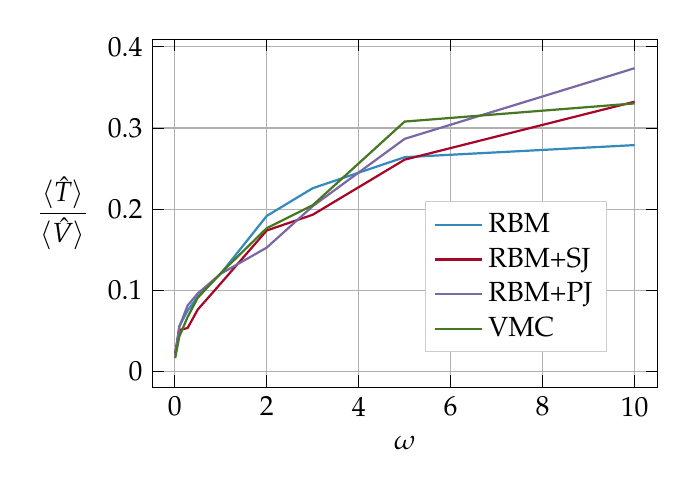
\begin{tikzpicture}

\begin{axis}[
legend cell align={left},
legend style={at={(0.9,0.1)}, anchor=south east, draw=white!80.0!black},
title style={yshift=-1.5ex},
%tick align=outside,
tick pos=both,
x grid style={white!69.01960784313725!black},
xlabel={\(\displaystyle \omega\)},
width=8cm,
height=6cm,
xmajorgrids,
xmin=-0.4895, xmax=10.4995,
xtick style={color=black},
y grid style={white!69.01960784313725!black},
ylabel style={rotate=-90.0},
ylabel={\(\displaystyle \frac{\langle\hat{T}\rangle}{\langle\hat{V}\rangle}\)},
ymajorgrids,
%ymin=-0.03, ymax=0.7,
ytick style={color=black}
]
\addplot [thick, color0]
table {%
	0.01 0.0202855736090596
	0.1 0.0558188176084186
	0.28 0.0748673013733255
	0.5 0.092181964299863
	1 0.120447174205168
	2 0.191577362501107
	3 0.2257693437
	5 0.263982205508037
	10 0.278872126802915
};
\addlegendentry{RBM}
\addplot [thick, color1]
table {%
	0.01 0.0224807471735212
	0.1 0.0510365183964855
	0.28 0.0535270823545204
	0.5 0.0761996706229769
	1 0.108428284656055
	2 0.17366909653192
	3 0.19307880632568
	5 0.260942252768941
	10 0.332349732889548
};
\addlegendentry{RBM+SJ}
\addplot [thick, color2]
table {%
	0.01 0.0198390540318607
	0.1 0.0550696242390316
	0.28 0.0812272164373049
	0.5 0.0960548685344326
	1 0.120346512979882
	2 0.152555093728466
	3 0.20363356015151
	5 0.286590458917023
	10 0.373618884667807
};
\addlegendentry{RBM+PJ}
\addplot [thick, color3]
table {%
	0.01 0.0164511376657391
	0.1 0.0430938843433643
	0.28 0.067074638154502
	0.5 0.0907330085826954
	1 0.121087634122869
	2 0.176534004132603
	3 0.20481414099371
	5 0.307872099467483
	10 0.330233868695407
};
\addlegendentry{VMC}
\end{axis}
\end{tikzpicture}
		%\caption{$N=20$}
	\end{figure}
}

\note{
	\begin{itemize}
		\item Still looking at 20 electrons $\rightarrow$ Distribution between kinetic and potential energy 
		\item Low frequency $\rightarrow$ Potential energy dominates over kinetic energy
		\item High frequency $\rightarrow$ Ansätze differ $\rightarrow$ Different electron configurations
	\end{itemize}
}

\mframe{One-body Density}{Number of electrons: $N=20$. Frequency: $\omega=1.0$.}{
	\begin{figure}
		\centering
		\captionsetup[subfigure]{labelformat=empty}
		\subfloat{\raisebox{1cm}{\rotatebox[origin=t]{90}{RBM}}}\hspace{0.cm}
		\subfloat{{\includegraphics[width=3cm]{../plots/int1/onebody2/2D/20P/1.000000w/RBM_ADAM_MC1048576.png}}}\hspace{0.5cm}
		\subfloat{\raisebox{1cm}{\rotatebox[origin=t]{90}{RBM+SJ}}}\hspace{0.cm}
		\subfloat{{\includegraphics[width=3cm]{../plots/int1/onebody2/2D/20P/1.000000w/RBMSJ_ADAM_MC1048576.png}}}\\
		\subfloat{\raisebox{1cm}{\rotatebox[origin=t]{90}{RBM+PJ}}}\hspace{0.cm}
		\subfloat{{\includegraphics[width=3cm]{../plots/int1/onebody2/2D/20P/1.000000w/RBMPJ_ADAM_MC1048576.png}}}\hspace{0.5cm}
		\subfloat{\raisebox{1cm}{\rotatebox[origin=t]{90}{VMC}}}\hspace{0.cm}
		\subfloat{{\includegraphics[width=3cm]{../plots/int1/onebody2/2D/20P/1.000000w/VMC_ADAM_MC1048576.png}}}
		%\caption{$N=20$, $\omega=1.0$}
	\end{figure}
}

\note{
	\begin{itemize}
		\item One-body density describes how electrons distribute throughout the space
		\item Ansätze with Jastrow factor almost identical
		\item RBM provides more distinct peaks $\rightarrow$ model the electrons
	\end{itemize}
}

\mframe{Two-body Density}{Number of electrons: $N=20$. Frequency: $\omega=1.0$.}{
	\begin{figure}
		\centering
		\captionsetup[subfigure]{labelformat=empty}
		\subfloat{\raisebox{1cm}{\rotatebox[origin=t]{90}{RBM}}}\hspace{0.cm}
		\subfloat{{\includegraphics[width=3cm]{../plots/int1/twobody/2D/20P/1.000000w/RBM_ADAM_MC1048576.png}}}\hspace{0.5cm}
		\subfloat{\raisebox{1cm}{\rotatebox[origin=t]{90}{RBM+SJ}}}\hspace{0.cm}
		\subfloat{{\includegraphics[width=3cm]{../plots/int1/twobody/2D/20P/1.000000w/RBMSJ_ADAM_MC1048576.png}}}\\
		\subfloat{\raisebox{1cm}{\rotatebox[origin=t]{90}{RBM+PJ}}}\hspace{0.cm}
		\subfloat{{\includegraphics[width=3cm]{../plots/int1/twobody/2D/20P/1.000000w/RBMPJ_ADAM_MC1048576.png}}}\hspace{0.5cm}
		\subfloat{\raisebox{1cm}{\rotatebox[origin=t]{90}{VMC}}}\hspace{0.cm}
		\subfloat{{\includegraphics[width=3cm]{../plots/int1/twobody/2D/20P/1.000000w/VMC_ADAM_MC1048576.png}}}
		%\caption{$N=20$, $\omega=1.0$}
	\end{figure}
}

\note{
	\begin{itemize}
		\item Two-body density describes how the electrons distribute pairwise
		\item The same can be observed here, where RBM stands out
	\end{itemize}
}

\mframe{Low-frequency Dots}{Number of electrons: $N$. Frequency: $\omega=0.1$.}{
	\begin{figure}
		\centering
		\captionsetup[subfigure]{labelformat=empty}
		\subfloat{\raisebox{1cm}{\rotatebox[origin=t]{90}{RBM}}}\hspace{0.1cm}
		\subfloat{{\includegraphics[width=3cm]{../plots/int1/onebody2/2D/2P/0.100000w/RBM_ADAM_MC1048576.png}}}\hspace{-0.cm}
		\subfloat{{\includegraphics[width=3cm]{../plots/int1/onebody2/2D/6P/0.100000w/RBM_ADAM_MC1048576.png}}}\hspace{-0.cm}
		\subfloat{{\includegraphics[width=3cm]{../plots/int1/onebody2/2D/12P/0.100000w/RBM_ADAM_MC1048576.png}}}\\ [-0.cm]
		
		\subfloat{\raisebox{1cm}{\rotatebox[origin=t]{90}{VMC}}}\hspace{0.1cm}
		\subfloat[$N=2$]{{\includegraphics[width=3cm]{../plots/int1/onebody2/2D/2P/0.100000w/VMC_ADAM_MC1048576.png}}}\hspace{-0.cm}
		\subfloat[$N=6$]{{\includegraphics[width=3cm]{../plots/int1/onebody2/2D/6P/0.100000w/VMC_ADAM_MC1048576.png}}}\hspace{-0.cm}
		\subfloat[$N=12$]{{\includegraphics[width=3cm]{../plots/int1/onebody2/2D/12P/0.100000w/VMC_ADAM_MC1048576.png}}}
		%\caption{$\omega=0.1$}
	\end{figure}
}

\note{
	\begin{itemize}
		\item Move on to low=frequency dots
		\item Interesting since RBM gives very different profiles from VMC
		\item $N$=peaks
		\item Indicates very localized electrons
		\item Indicates that energy is not the best way of evaluate an ansatz
	\end{itemize}
}

\mframe{Computational Cost}{Number of electrons: $N$.}{
	\begin{figure}
		\centering 
		% This file was created by matplotlib2tikz v0.7.4.
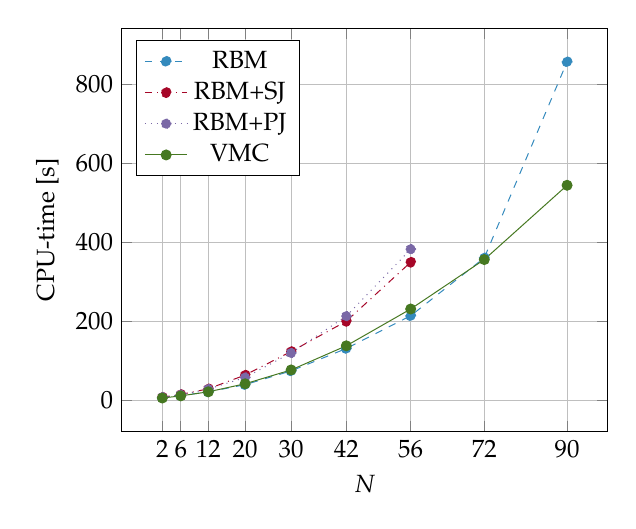
\begin{tikzpicture}[scale=0.9]

\begin{axis}[name=2D, xlabel=$N$, ylabel={CPU-time [s]}, grid=major, legend pos=north west, xtick=data] 
\addplot[color=color0,mark=oplus*, dashed] coordinates { 
	(2,6.05)
	(6,11.25)
	(12,20.53) 
	(20,38.99) 
	(30,73.73) 
	(42,130.49) 
	(56,213.47)
	(72,360.22)
	(90,856.84) }; 
\addlegendentry{RBM};

\addplot[color=color1,mark=oplus*, dash dot] coordinates { 
	(2,7.12) 
	(6,14.07) 
	(12,28.42) 
	(20,63.27) 
	(30,122.93) 
	(42,199.60)
	(56,349.22)}; 
\addlegendentry{RBM+SJ};

\addplot[color=color2,mark=oplus*, dotted] coordinates { 
	(2,7.26)
	(6,13.50)
	(12,27.68)
	(20,57.09) 
	(30,119.17) 
	(42,212.53) 
	(56,382.13) }; 
\addlegendentry{RBM+PJ};

\addplot[color=color3,mark=oplus*] coordinates { 
	(2,5.11)
	(6,10.51)
	(12,20.85) 
	(20,41.20) 
	(30,76.26) 
	(42,137.39) 
	(56,230.63)
	(72,355.81)
	(90,544.03) }; 
\addlegendentry{VMC};
\end{axis}
\end{tikzpicture}
	\end{figure} 
}

\note{
	\begin{itemize}
		\item RBM and VMC pairwise
		\item RBM explodes for large systems $\rightarrow$ 10,000 parameters vs 2
		\item RBM+PJ and RBM+SJ pairwise most computationally intensive $\rightarrow$ No point to choose RBM+PJ considering the other results
	\end{itemize}
}
\titleframe{Conclusions}

\note{Now we will address some brief conclusions. }

\mframe{Conclusions}{}{
	\begin{itemize}
		\setlength\itemsep{2em}
		\item The RBM ansatz is able to account for most of the correlations
		\item The RBM+PJ ansatz might give a better ground state estimate of small quantum dots, compared to the traditional VMC ansatz
		\item For larger quantum dots, RBM+PJ gives slightly larger energy than VMC
		\item The energy distribution is different for the different methods, indicating different electron configurations.
		\item The ground state energy might not be the best way to evaluate the various ansätze
	\end{itemize}
}

\note{We have seen that the RBM method usually provides energies lower than the Hartree-Fock limit. This indicates that it is able to account for most of the electron-electron correlations. When adding a Padé-Jastrow factor to the RBM ansatz, it usually provides lower energy than the VMC ansatz for the smallest systems. This is an important result, as it indicates that RBM+PJ is able to provide a better estimate of the ground state energy than VMC. However, for larger quantum dots, VMC gives a slightly lower energy than RBM+PJ, which can be explained by the large number of variational parameters in the RBM+PJ ansatz. }

\note{Even though the energy is quite similar for the various methods, the ratio between kinetic and potential energy reveals that the distribution between kinetic and potential energy is different. To change the potential energy, the electron configuration has to be different, meaning that the various ansätze provide different particle positions. We have also observed that different ansätze provide very different electron density plots even when the energy is similar. This indicates that the energy might not be the best way to evaluate various ansätze. }

\mframe{Future Work}{}{
	\begin{itemize}
		\setlength\itemsep{3em}
		\item Investigate restricted Boltzmann machines with other architectures
		\item Pass more information to the restricted Boltzmann machine
		\item Apply the method on more complex systems
	\end{itemize}
}

\note{Even though we have investigated various restricted Boltzmann machine architectures and hyper parameter settings, there are still many things that should be investigated. Our results indicates that the number of hidden units used in the restricted Boltzmann machine might be too large. On the other hand, Carleo and Troyer consequently used a larger number of hidden nodes. 
\bigskip

We have only passed the electron coordinates to the Boltzmann machines. However, if we also pass the relative distances between the electrons, it might be able to model the electron-electron correlations more correctly. This was inspired by what Pfau et. al did. }

\note{Quantum dots are very simple systems, but the main application of this method is on systems where we don't have much information about the wave function. It is therefore obvious that it should be applied on more complex systems. It has shown that it can model electron-electron correlations, so it might be able to model three-body correlations as well, which is found in nuclear systems. }


\titleframe{Thank you!}

\note{Thank you all for listening! Since I have a few more minutes, I will show how the developed software can be used. }

\mframe{References}{}{
	\printbibliography
}

\appendix

% Backup slides
\mframe{Test}{Test}{TEST}
\mframe{Test}{Test}{TEST}
\mframe{Test}{Test}{TEST}

\end{document}